\graphicspath{{chapters/chapter4/img/}}

\chapter{Results and discussion}
\label{cha:results}

This chapter is meant to show and discuss the results obtained from the application of the methods introduced in \Cref{cha:methods}.

\section{LIWC and EmoLex comparison}
\label{sec:comparison}

Before going into the details, it is worth showing the comparison between the results obtained using Emolex and the ones with LIWC. In particular, we decided to use the z-score of the data obtained from the analysis of both of them.

\Cref{fig:en-emotions-liwc-comparison}, \Cref{fig:it-emotions-liwc-comparison}, and \Cref{fig:es-emotions-liwc-comparison} show how the course of the emotion/category pairs looks similar. Moreover, on several occasions the two lines overlap and, even if there is a gap, they generally tend to increase or decrease simultaneously. Instead, the differences are probably related to a different word/emotion (or word/category) association in the two dictionaries. Furthermore, they use a different set of words: for example, “pandemic”, “virus”, and “vaccine” are not present in LIWC, making it more general than EmoLex.

In any case, the results obtained from the comparison are particularly good for those languages, such as Catalan, where it is not possible to use LIWC due to the lack of appropriate dictionaries.

\begin{figure}[H]
	\centering
    	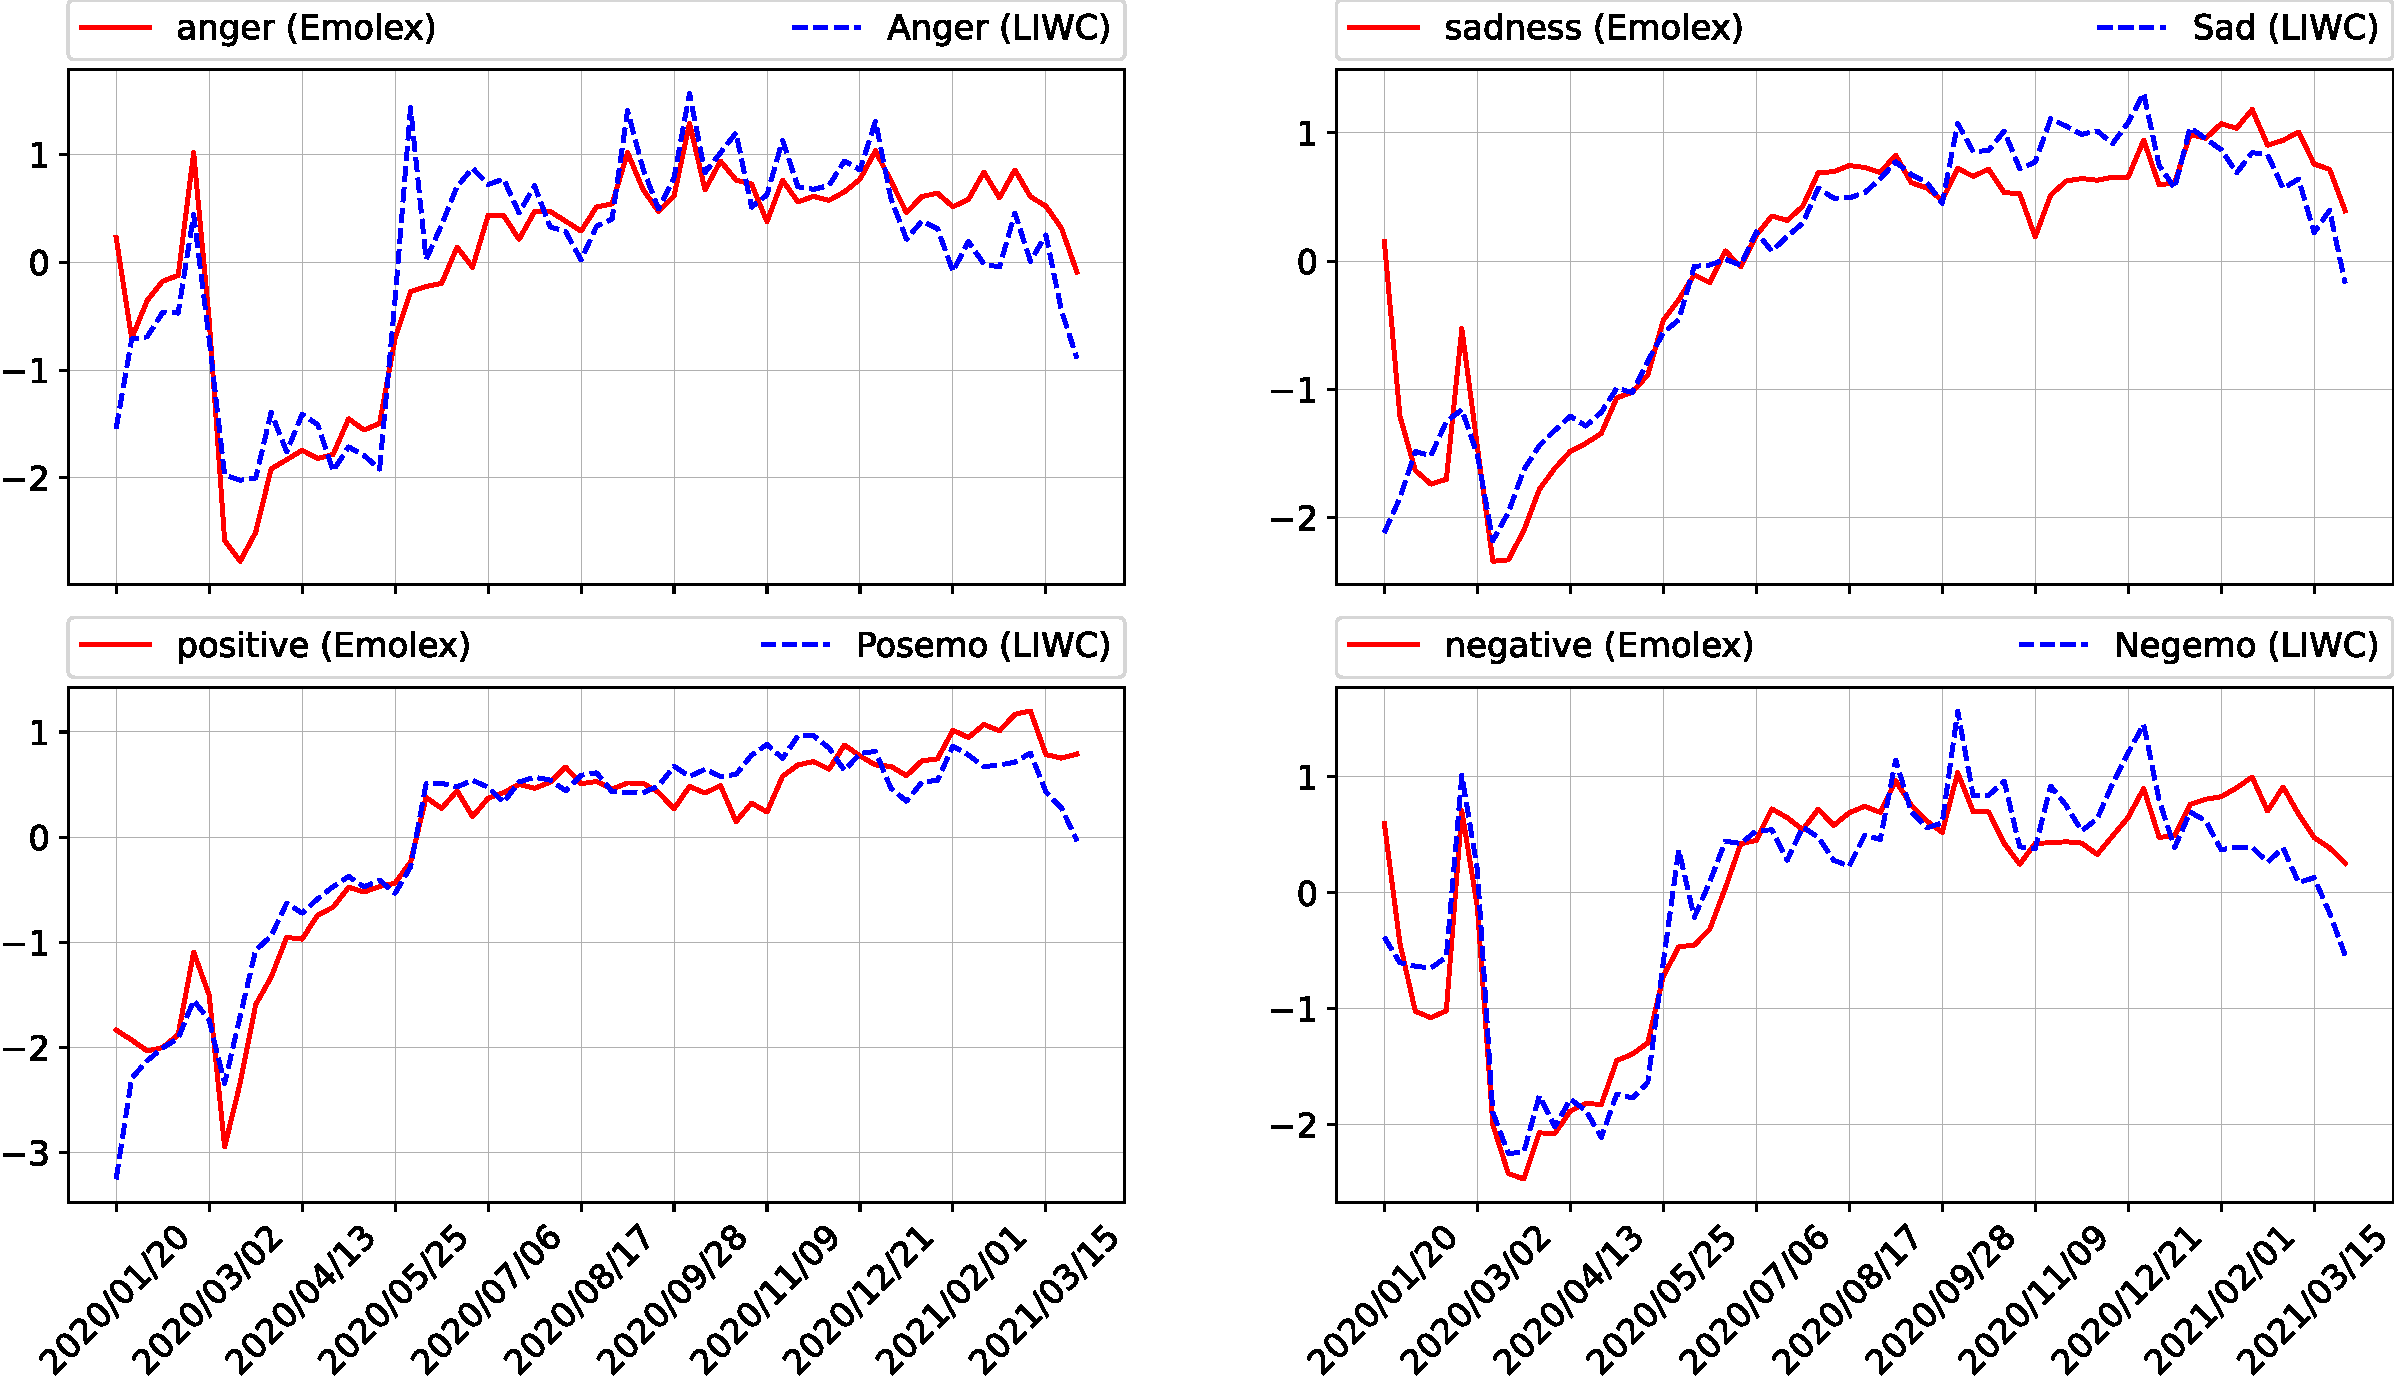
\includegraphics[scale=.3]{en_emotions_and_liwc_categories_comparison.svg}
    	\caption{Comparison between the z-score of the emotions and the z-score of the LIWC categories in the English tweets}
    	\label{fig:en-emotions-liwc-comparison}
    	
    	\vspace{.5cm}
    	
    	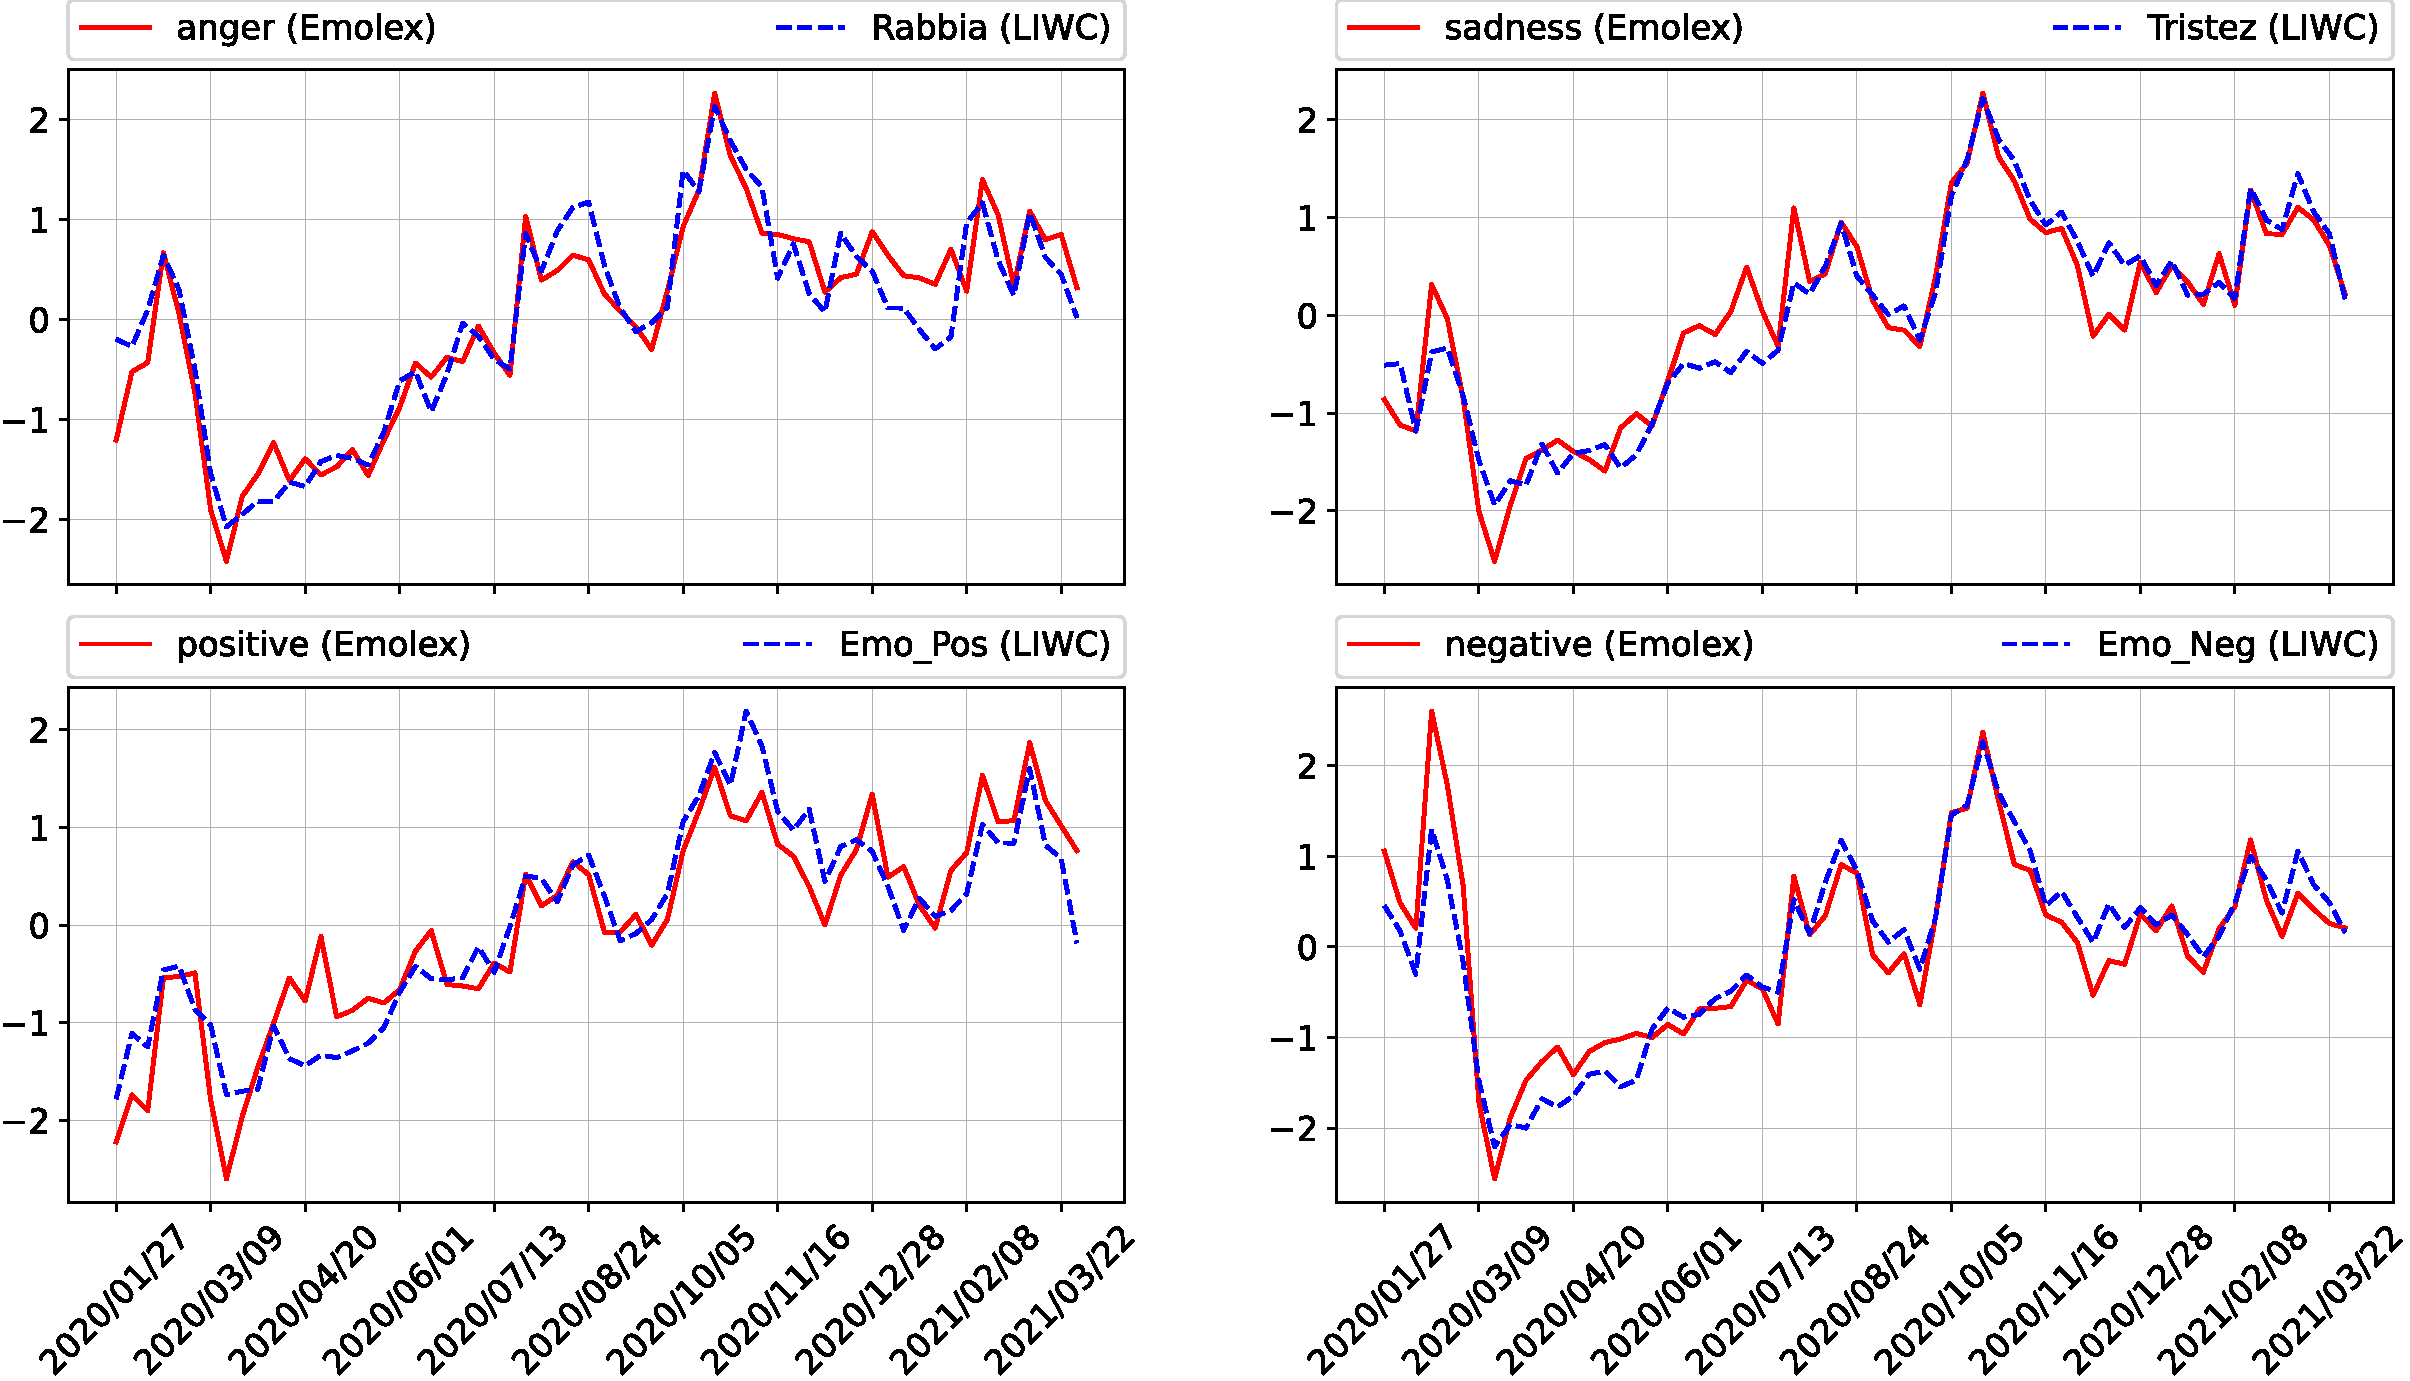
\includegraphics[scale=.3]{it_emotions_and_liwc_categories_comparison.svg}
    	\caption{Comparison between the z-score of the emotions and the z-score of the LIWC categories in the Italian tweets}
    	\label{fig:it-emotions-liwc-comparison}
    	
    	\vspace{.5cm}
    	
    	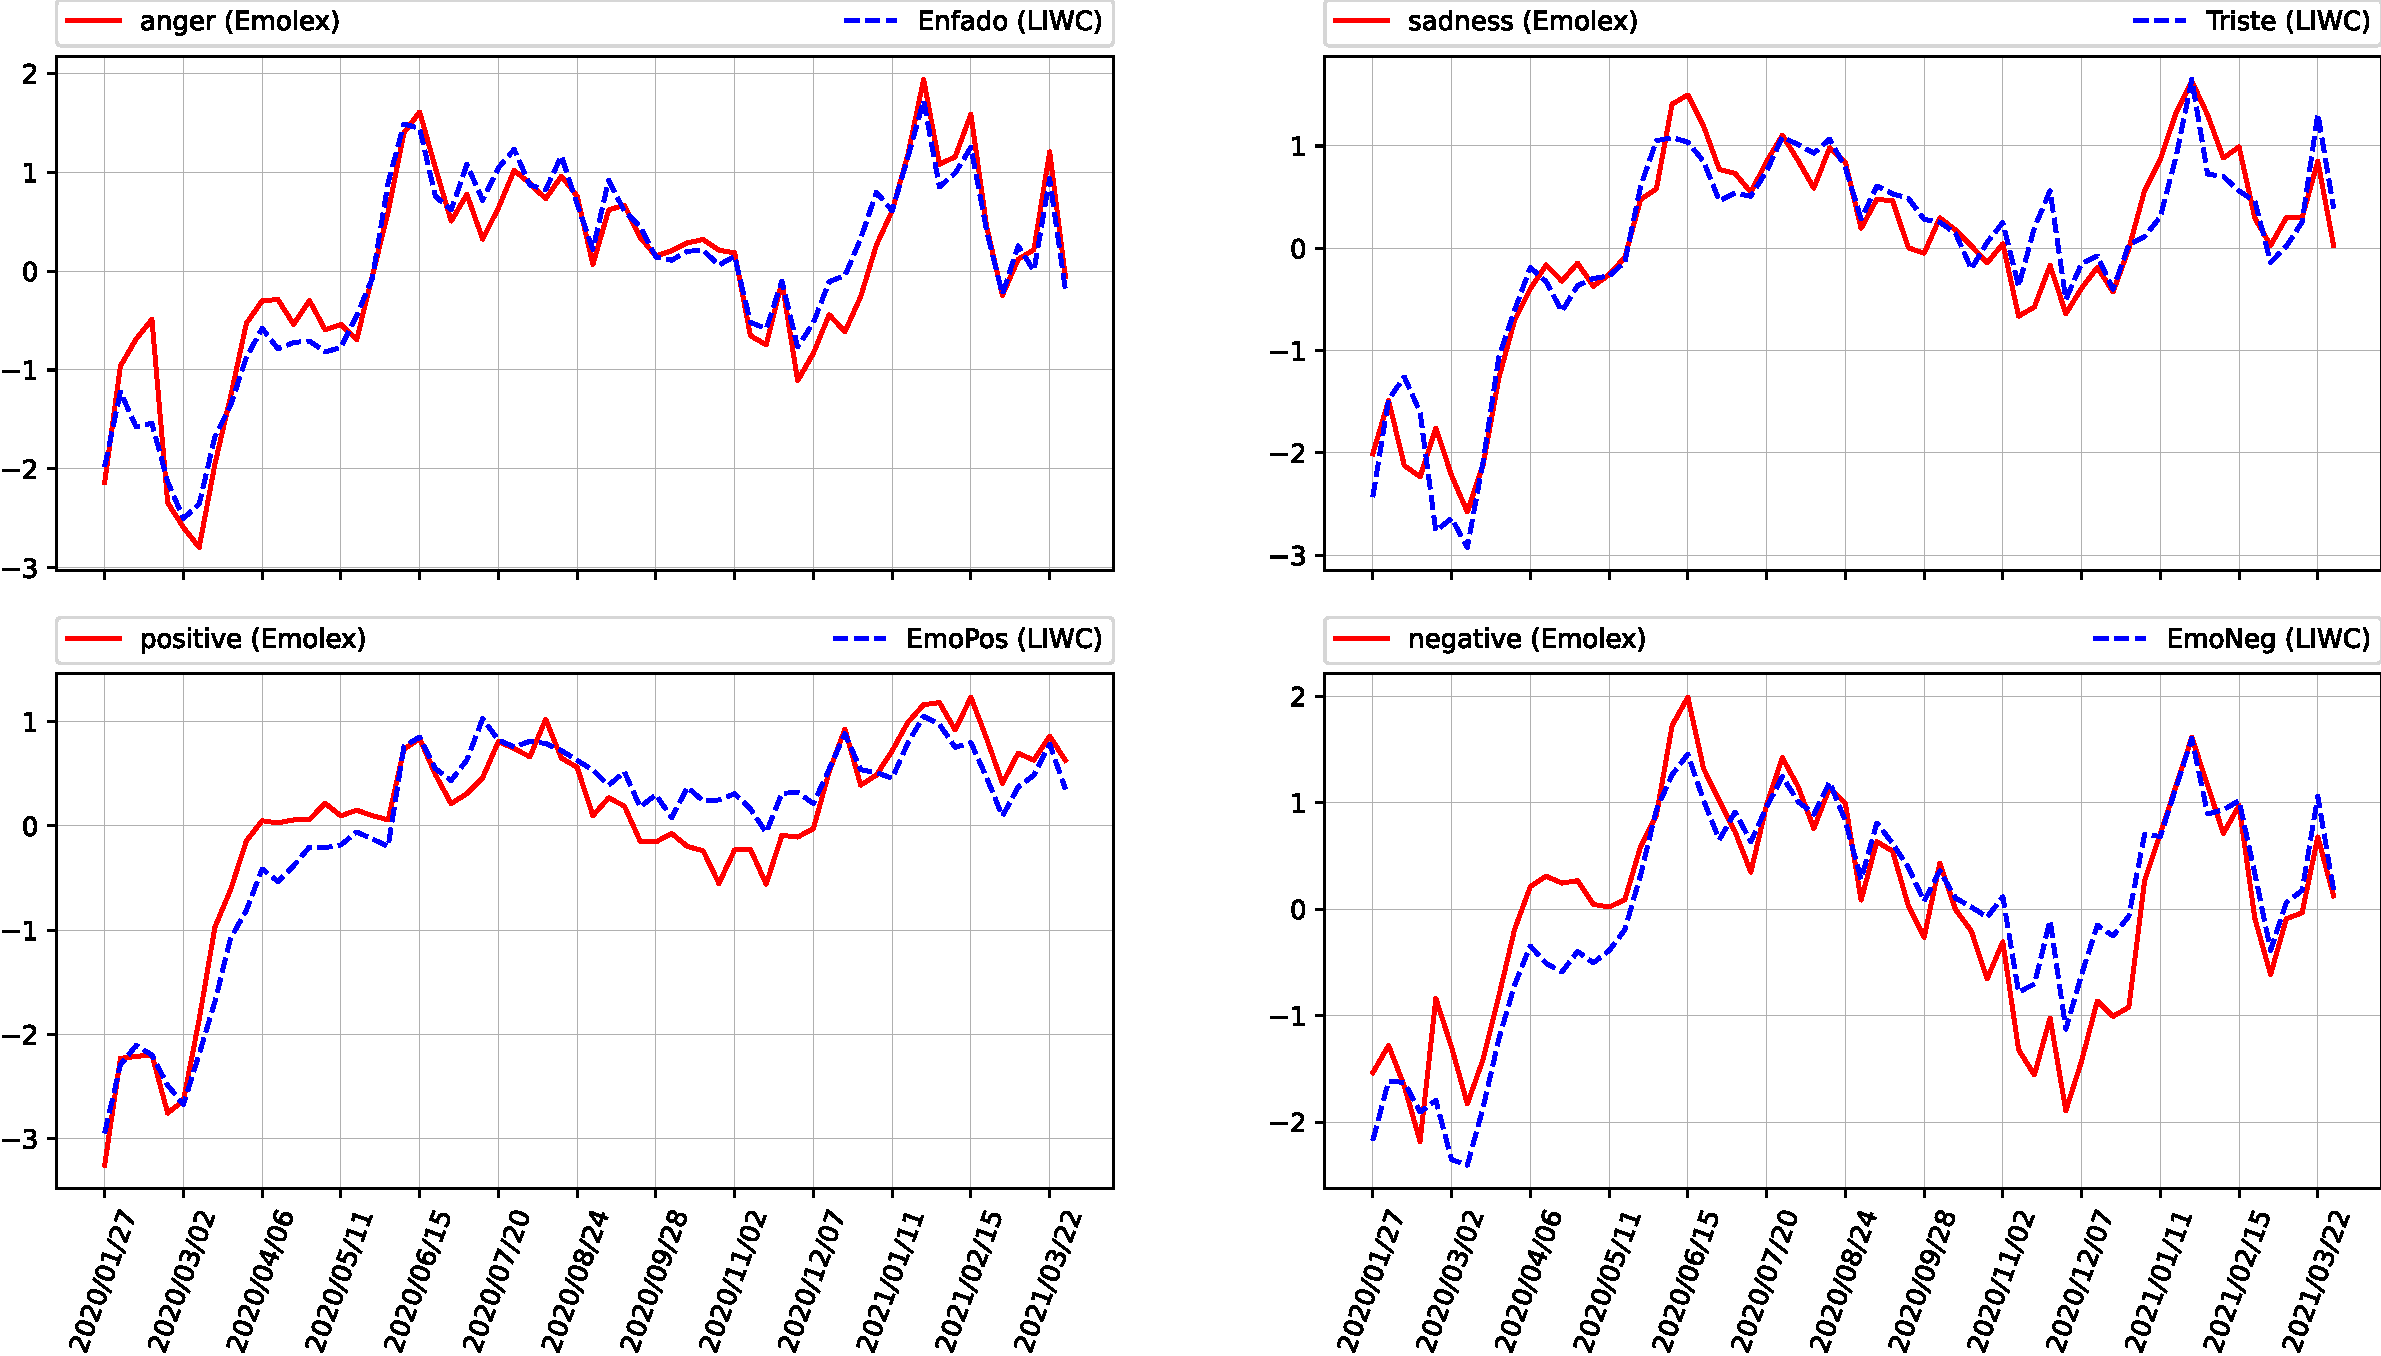
\includegraphics[scale=.3]{es_emotions_and_liwc_categories_comparison.svg}
    	\caption{Comparison between the z-score of the emotions and the z-score of the LIWC categories in the Spanish tweets}
    	\label{fig:es-emotions-liwc-comparison}
\end{figure}

\section{Emotion detection over time - by language}
\label{sec:emotion-by-language-results}

\begin{figure}[H]
	\centering
    	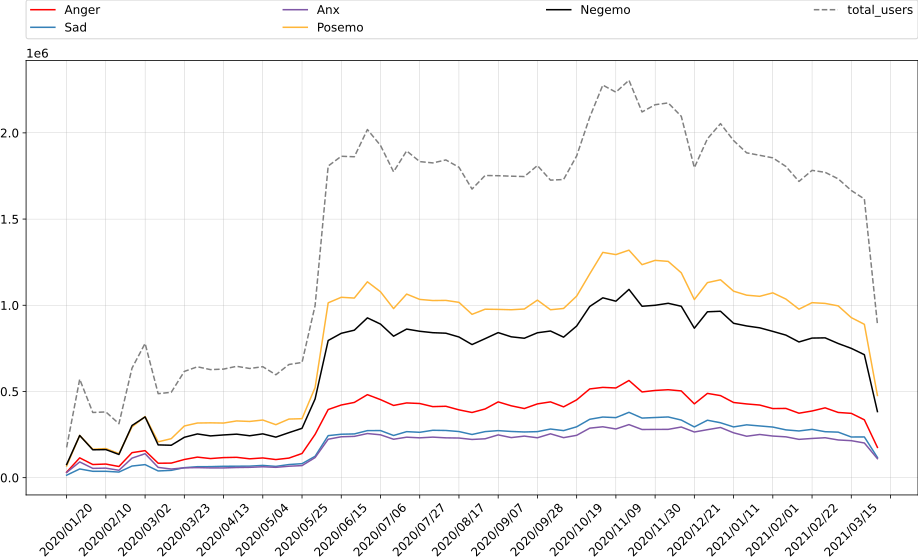
\includegraphics[scale=.35]{en_5_liwc_categories_abs.svg}
    	\caption{Number of weekly users per emotion in the English tweets}
    	\label{fig:en-5-liwc-categories-abs}
\end{figure}

\Cref{fig:en-5-liwc-categories-abs} displays the number of users that expressed a particular emotion in a given week, considering the English tweets. Instead, the gray dashed line indicates the number of users that posted at least one tweet during a week. The fact that the data collection migrated to AWS around June 2020, explains why the number of tweets almost doubled from 2020/06/01 to 2020/06/08.

\begin{figure}[H]
	\centering
    	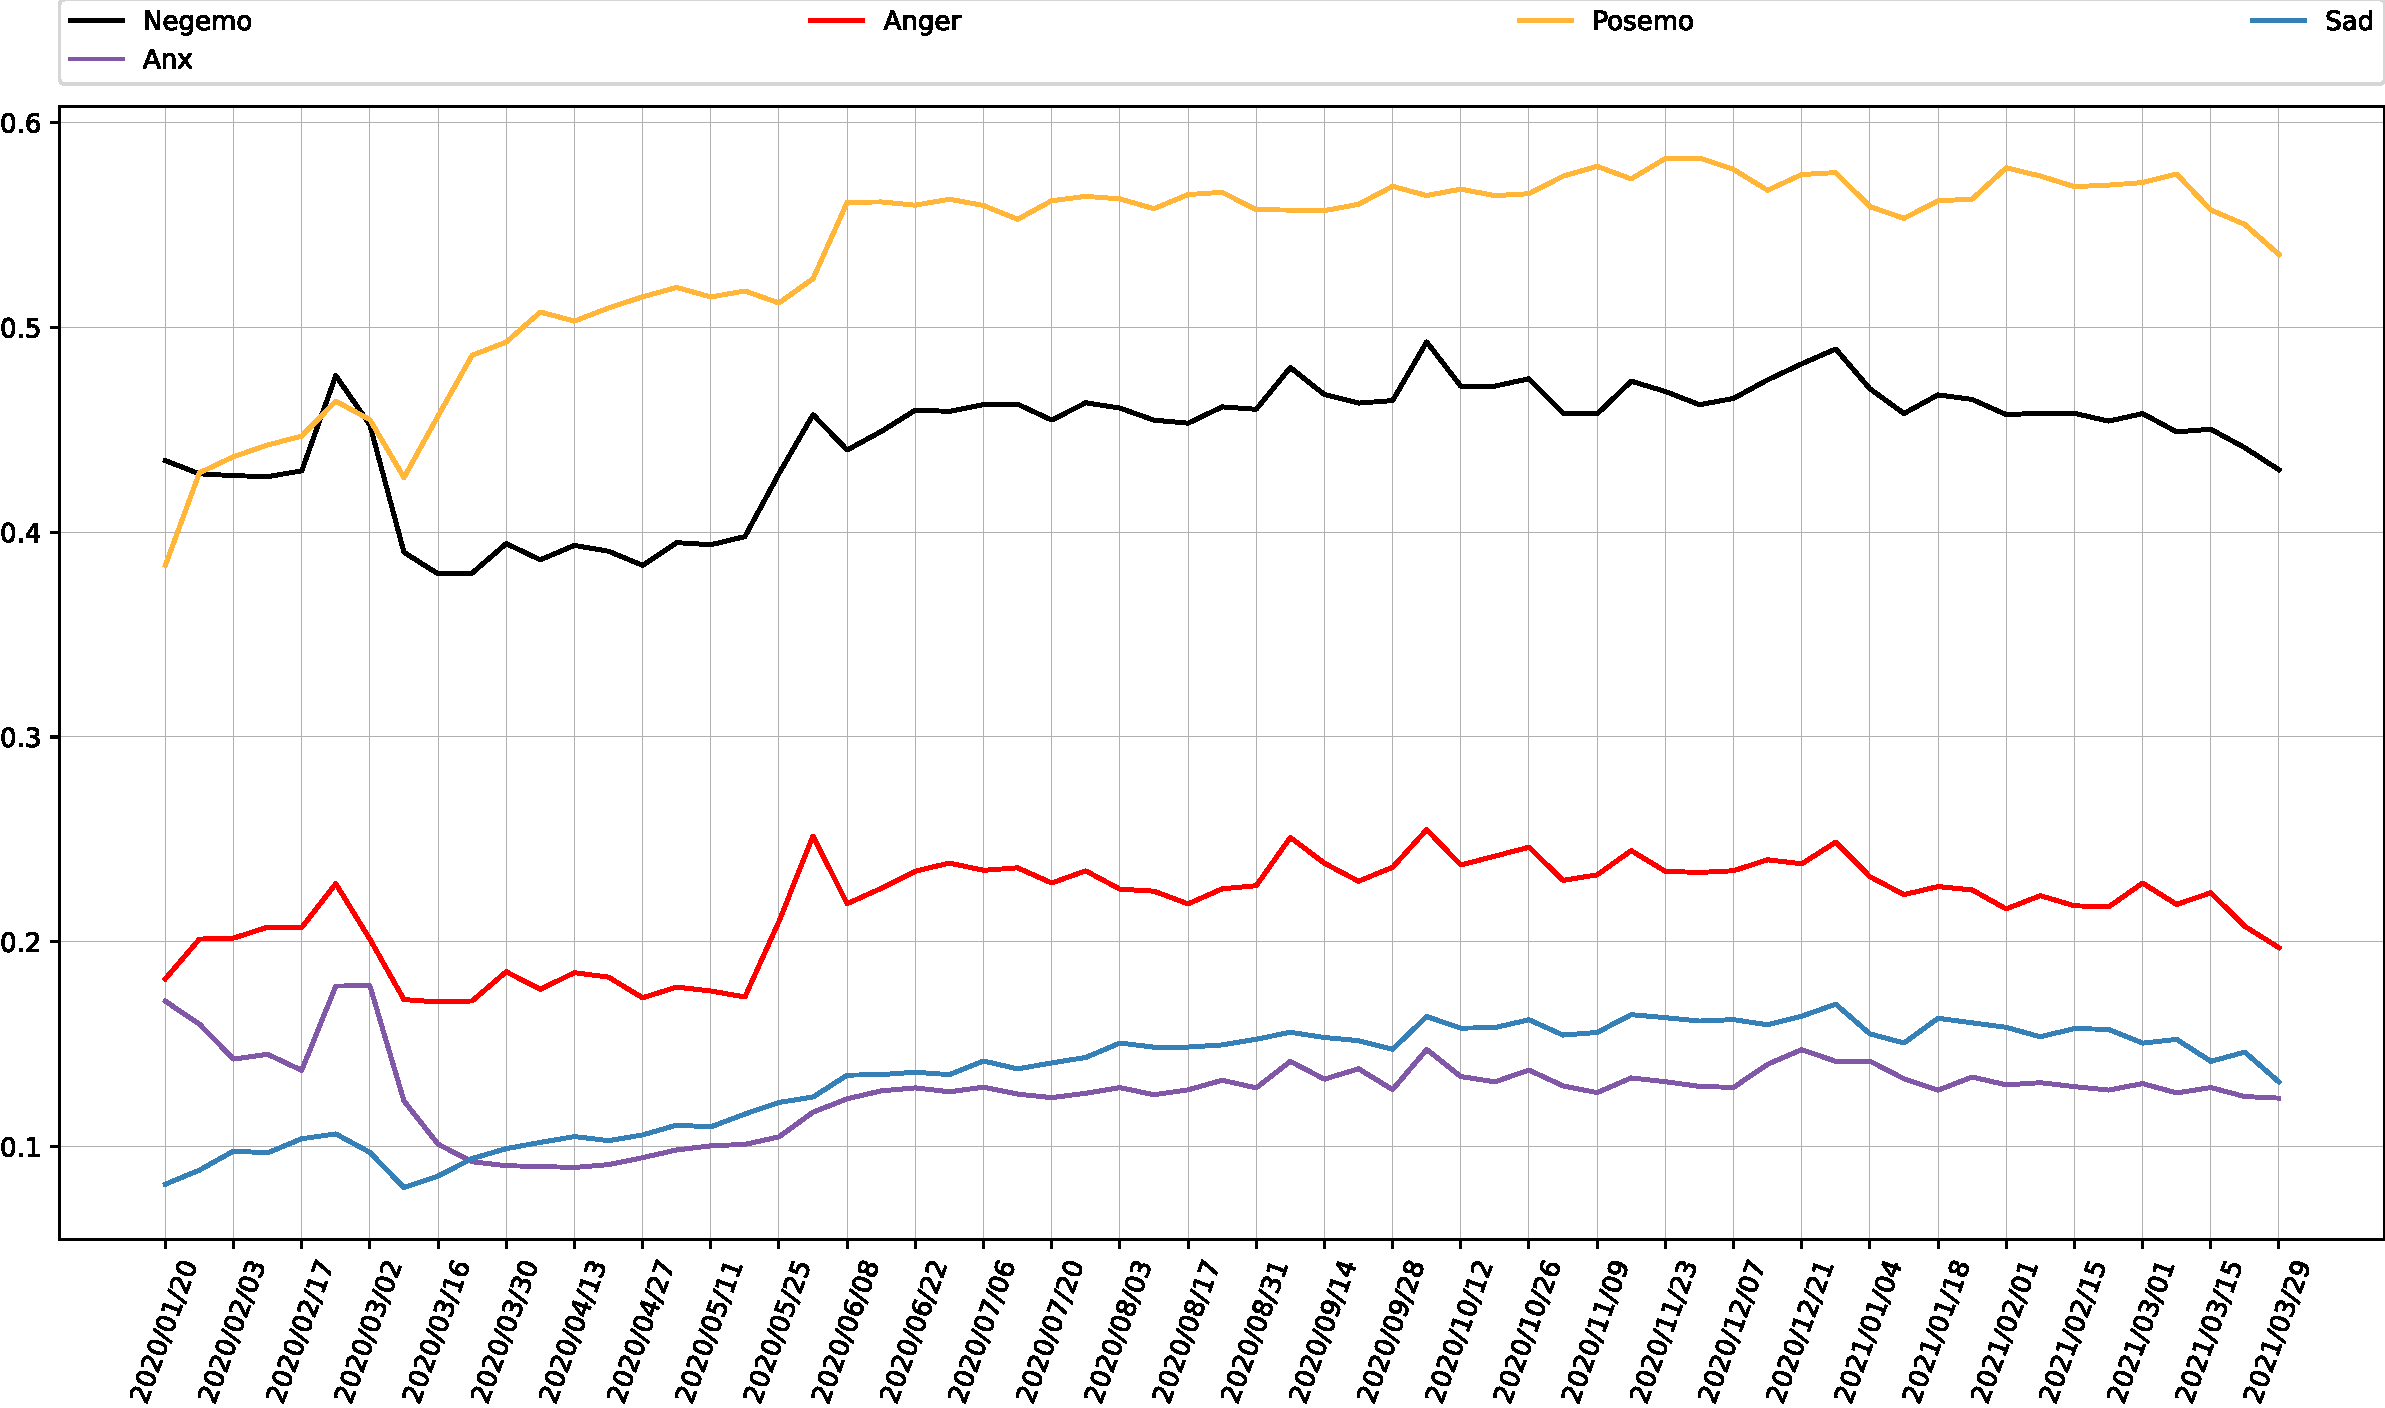
\includegraphics[scale=.35]{en_5_liwc_categories.svg}
    	\caption{Proportion of weekly users per emotion in the English tweets}
    	\label{fig:en-5-liwc-categories}
\end{figure}

\Cref{fig:en-5-liwc-categories} instead shows the proportion of users that expressed a particular emotion in a given week, considering the English tweets. Here we can notice some interesting results: first of all, we can see how the negative emotions course seems to be similar to the anger one, especially if we consider the peaks. However, this is not always the case: in fact, further analysis proved that Negemo can be seen as the combination of Anger, Sad, and Anx. Given its redundancy, we removed Negemo from the other graphics to achieve even better data visualization.

Secondly, there are some cases where all the emotions seem to have the same course. For the most, we can notice how, when negative emotions increase, positive emotions decrease (and vice versa). However, during the week starting on 2020/02/24, the proportion of users that expressed anger, sadness, anxiety, positive, and negative emotions raised. This probably happened because users during that time were particularly emotional and used several more words within a tweet.

\begin{figure}[H]
	\centering
    	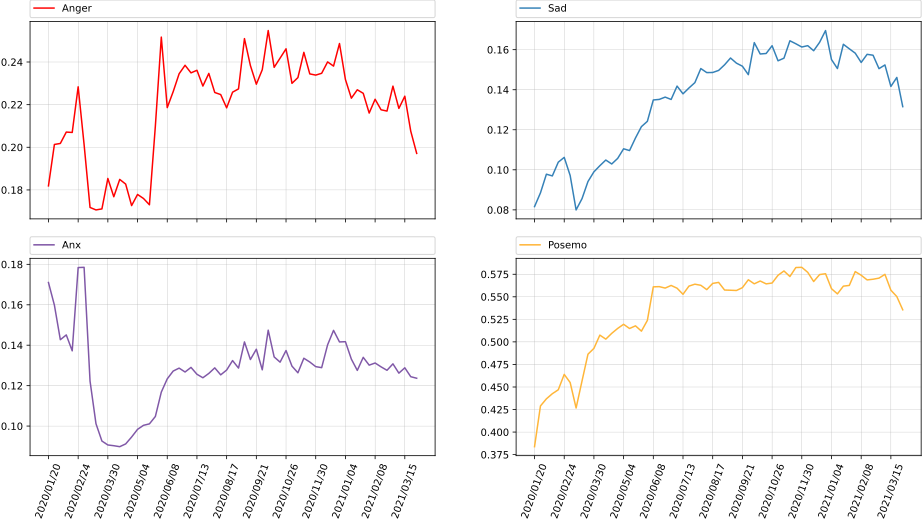
\includegraphics[scale=.35]{en_4_liwc_categories_subplots.svg}
    	\caption{Proportion of weekly users expressing a particular emotion in the English tweets}
    	\label{fig:en-4-liwc-categories-subplots}
\end{figure}

Before approaching the data normalization, we have also tried to divide the different emotions courses into subplots. If we take a look at \Cref{fig:en-4-liwc-categories-subplots}, both global (and local) maxima and minima are visible to the naked eye. However, the comparison between different emotions becomes really difficult.

\begin{figure}[H]
	\centering
    	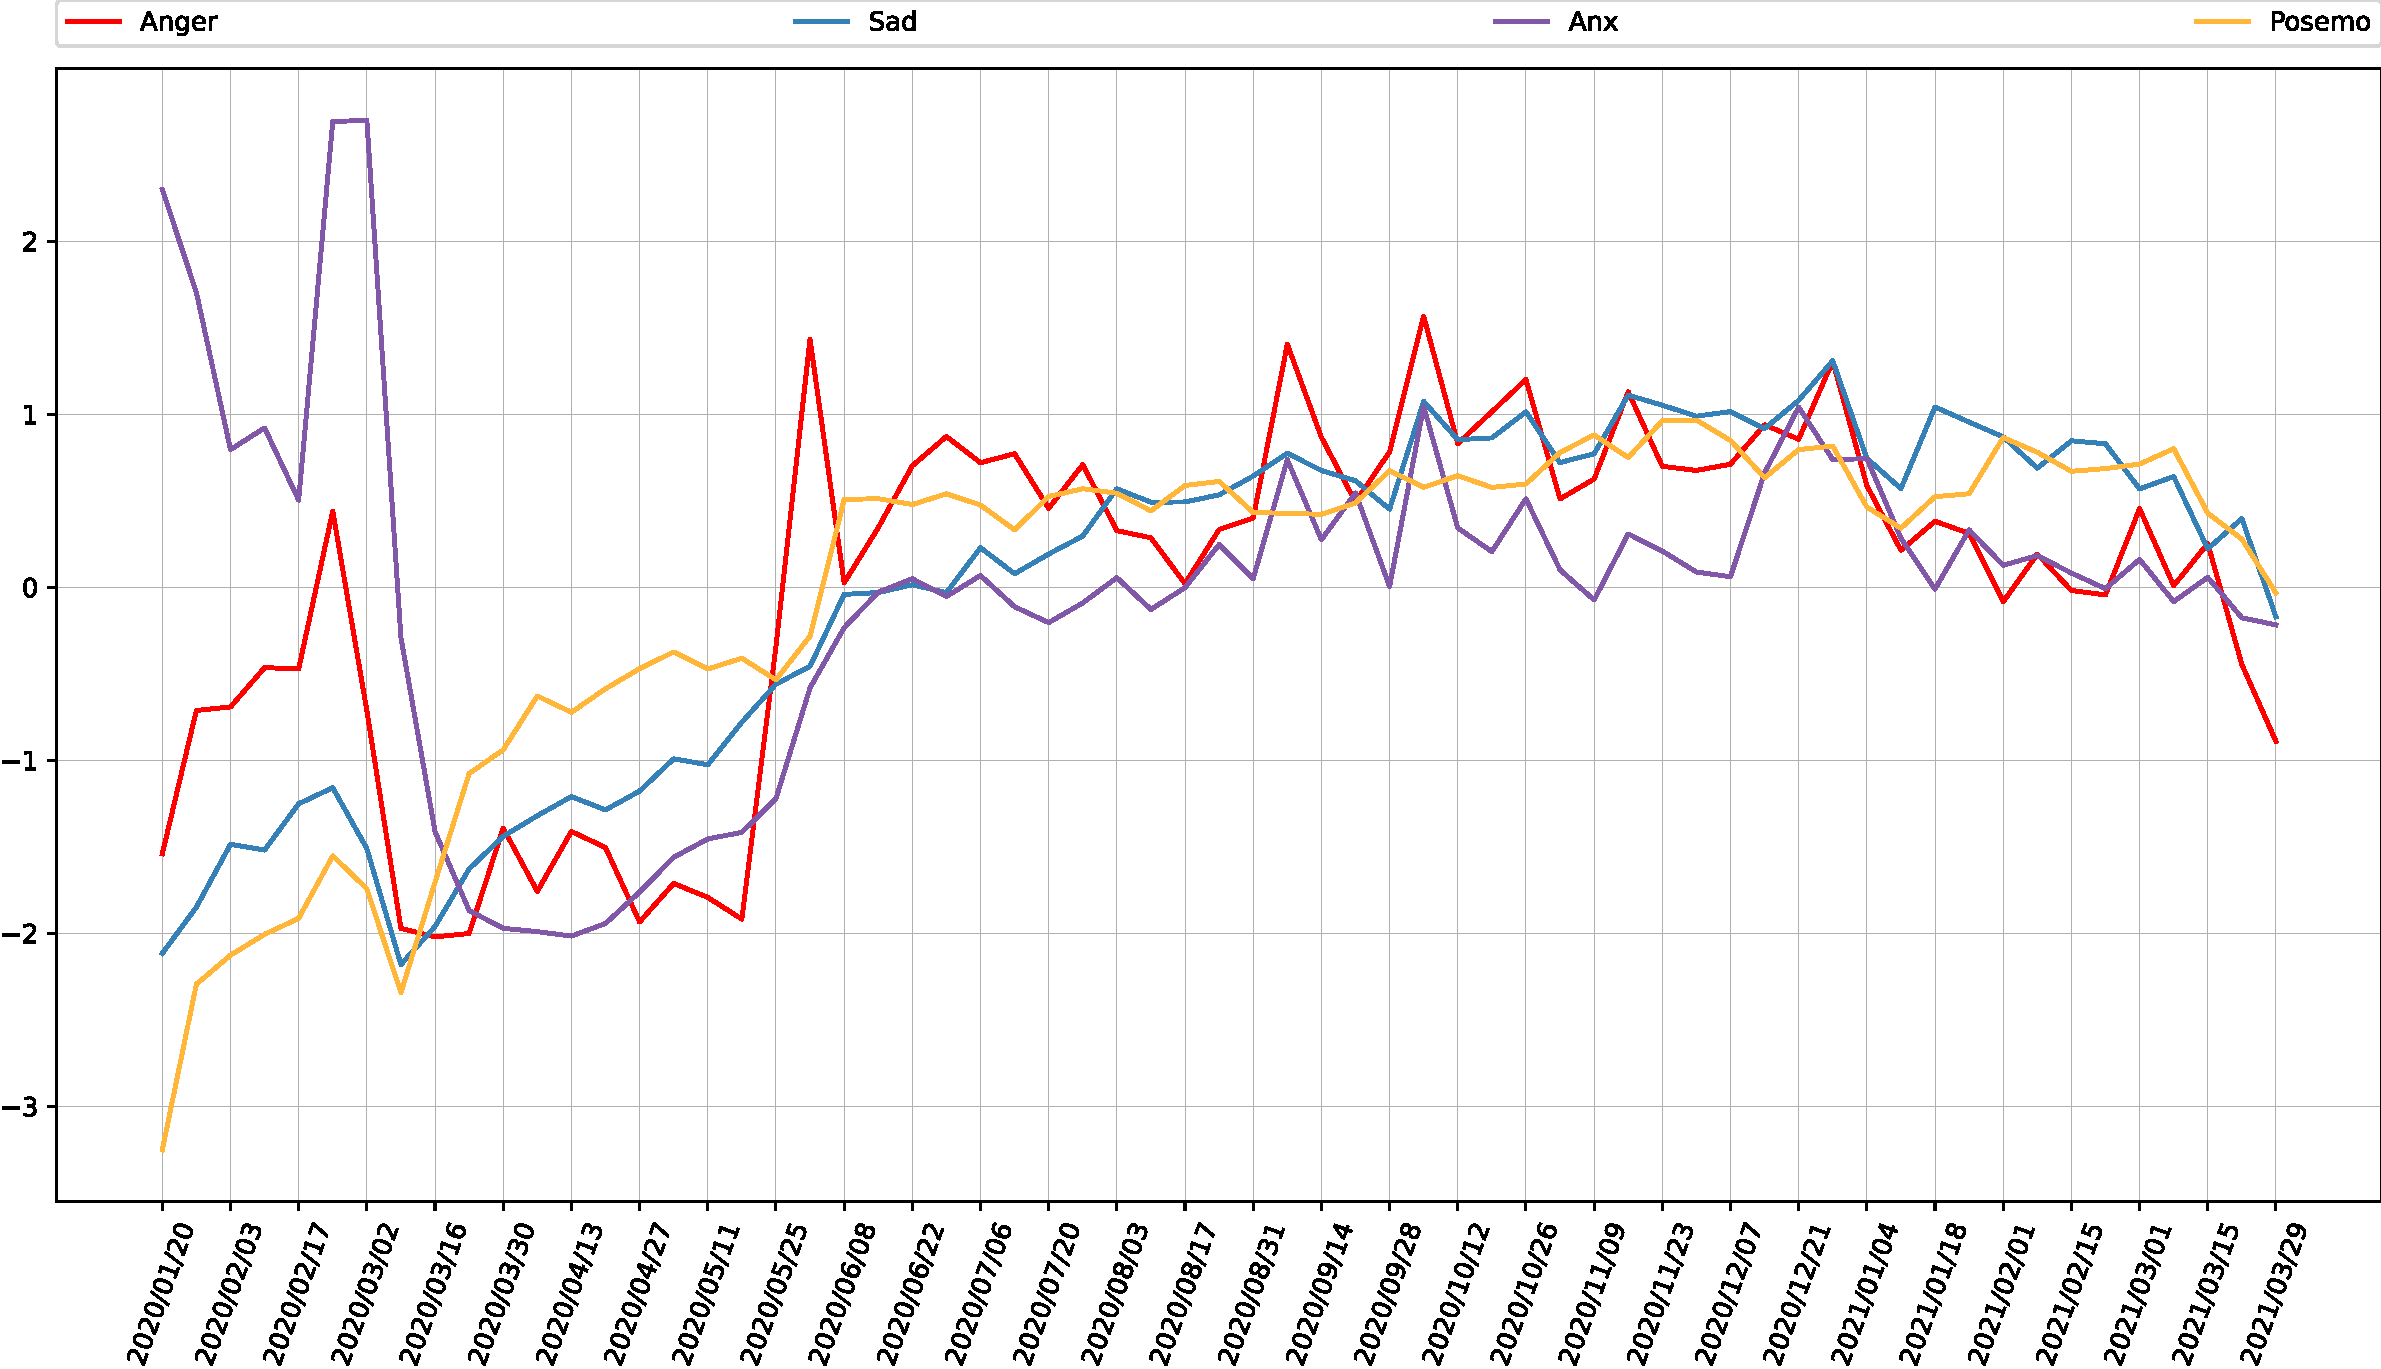
\includegraphics[scale=.35]{en_4_liwc_categories_standardized.svg}
    	\caption{Z-score of weekly users per emotion in the English tweets}
    	\label{fig:en-4-liwc-categories-std}
\end{figure}

The z-score instead proved to be a very useful data normalization. As we can see from \Cref{fig:en-4-liwc-categories-std}, not only peaks are noticeable even if we are considering the emotions altogether, but we can also understand which time frames are characterized by a greater (or lower) emotion value w.r.t. the mean value of that particular emotion. For example, it is possible to see that, starting on 2020/03/23, the proportion of users that expressed a positive emotion w.r.t. the mean value of positive emotion over the whole period surpassed all the other emotions w.r.t. their mean value over the whole period. For the same reason, we can see that the week starting on 2020/03/02 was characterized by a greater value of anxiety, even if in \Cref{fig:en-5-liwc-categories} the proportion of users that expressed a positive emotion is always higher.

From the comparison of the course of the emotions, we have manually selected some peaks (i.e. weeks) to understand which words associated with some emotions in our dictionaries were used the most. 

\begin{figure}[H]
	\centering
    	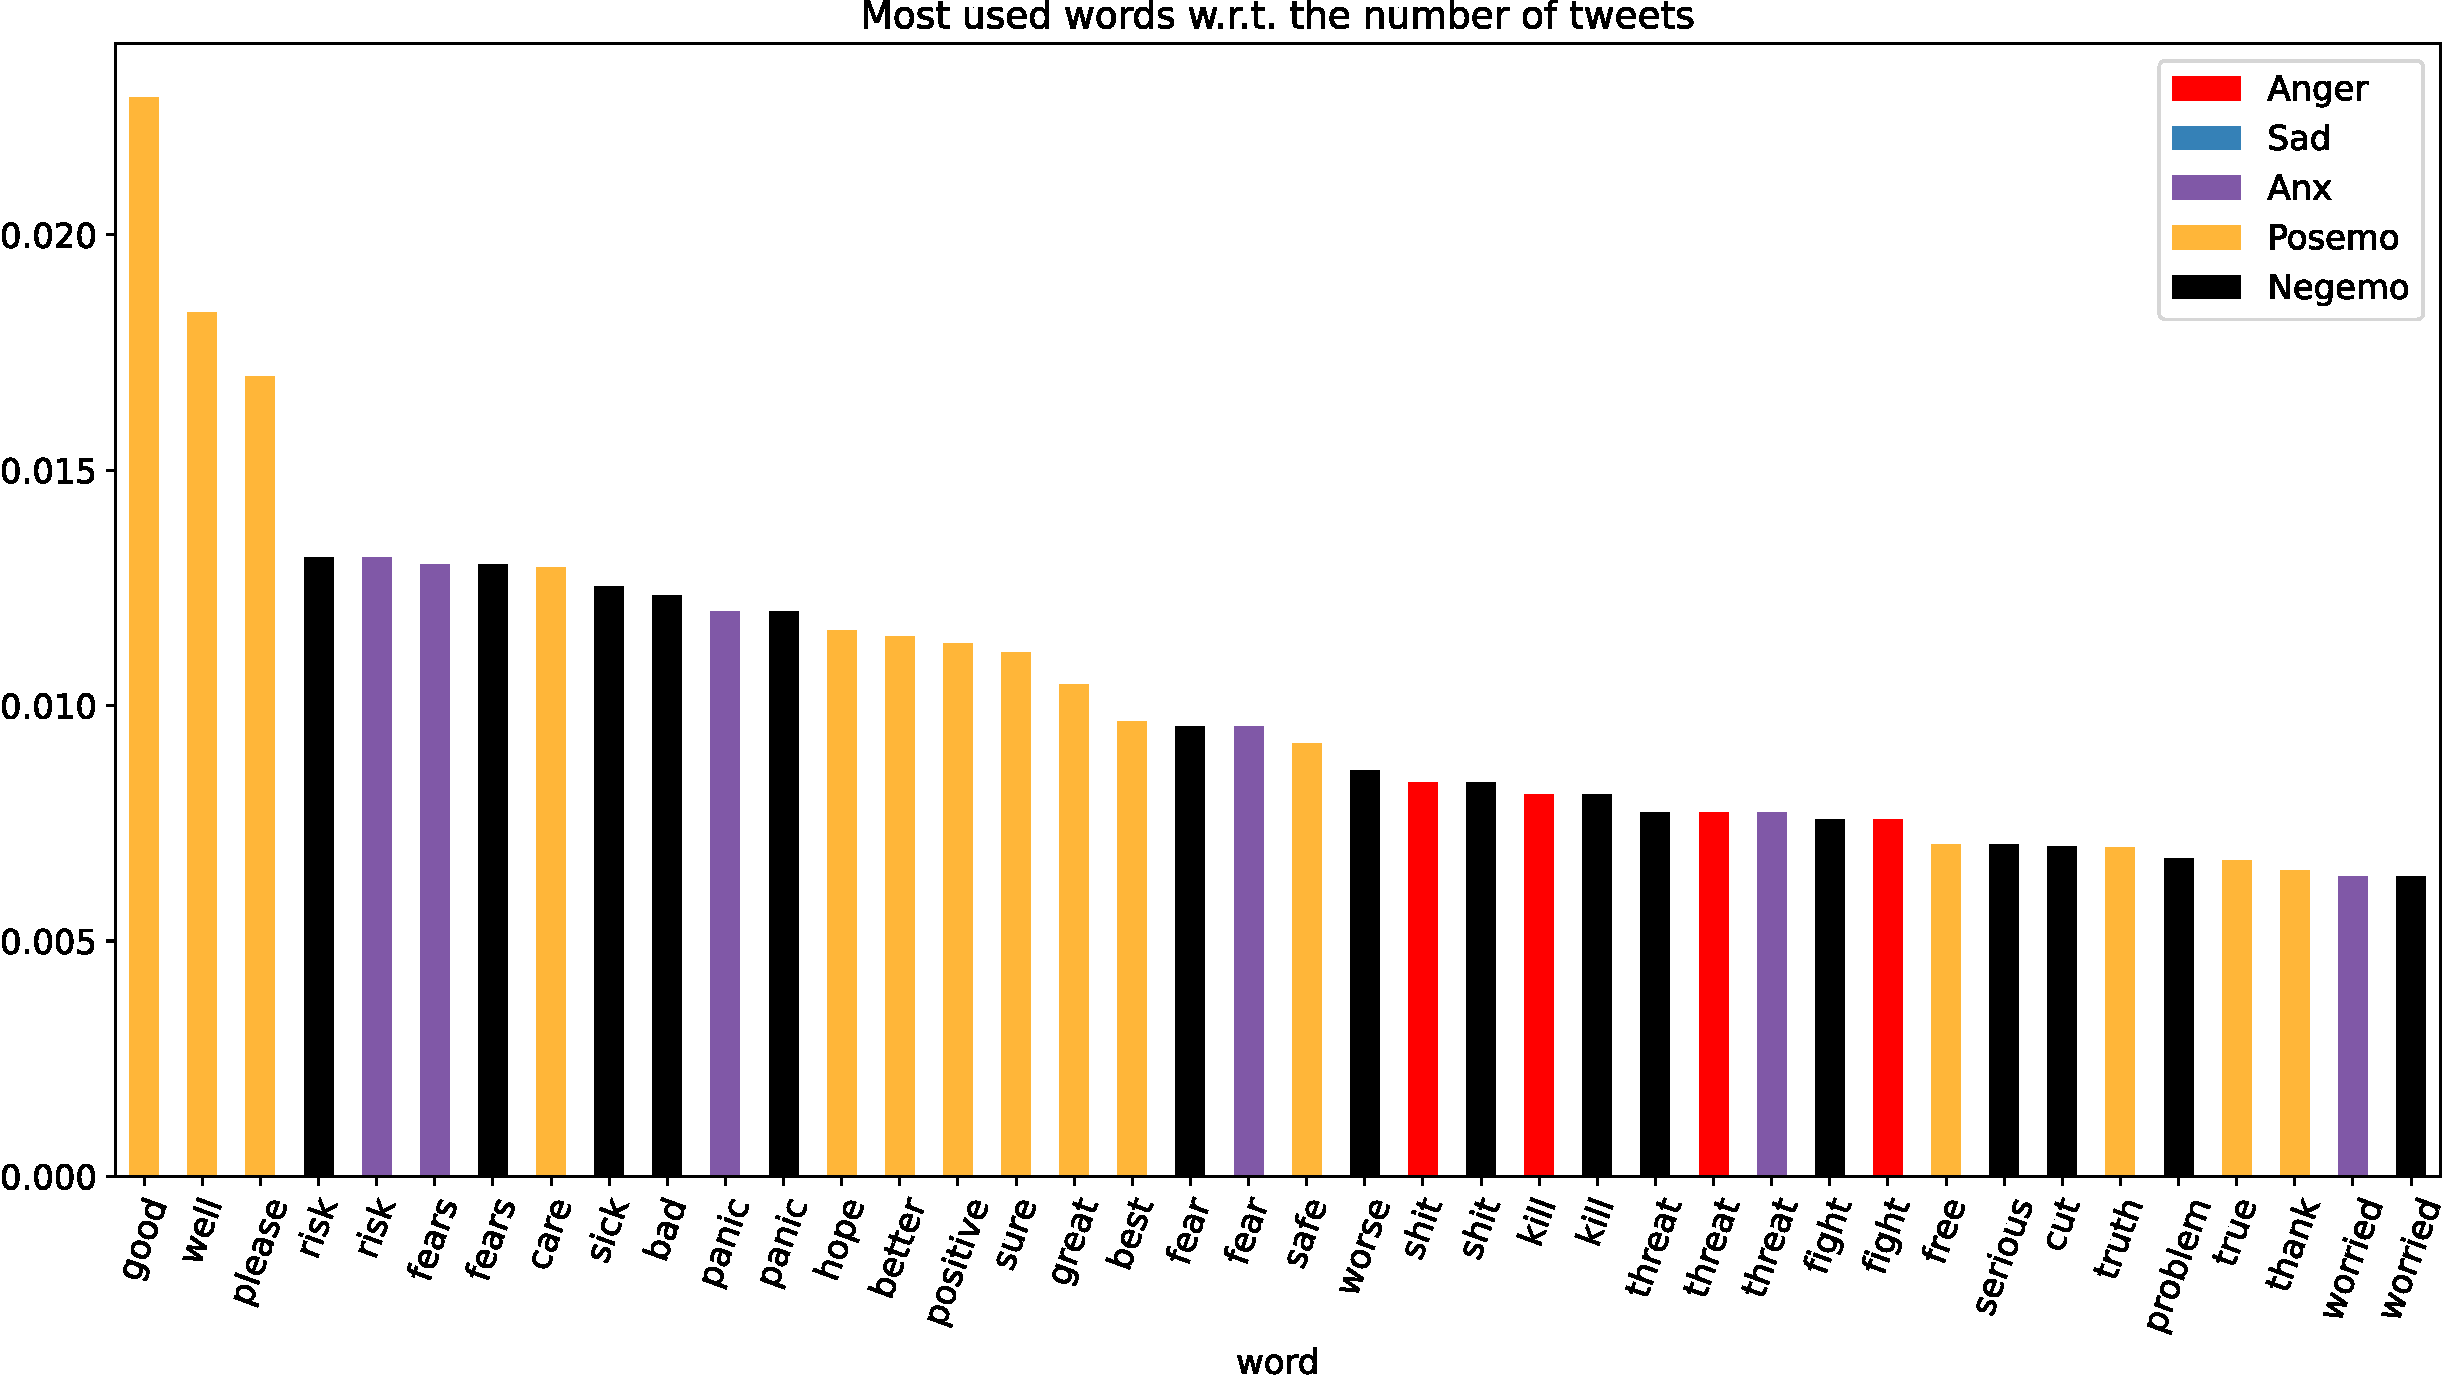
\includegraphics[scale=.32]{en_most_used_liwc_words_2020_02_24.svg}
    	\caption{Proportion of most used words on 2020/02/24 that express an emotion in the English tweets}
    	\label{fig:en-most-used-liwc-words-2020-02-24}
\end{figure}

\Cref{fig:en-most-used-liwc-words-2020-02-24} shows which are the 40 most used words in the English tweets during the week starting on 2020/02/24.

Here, we can that the majority of the words expressing a negative emotion are also associated with anger, sadness, or anxiety. This explains why we removed negative emotions from the other figures.

\begin{figure}[H]
	\centering
    	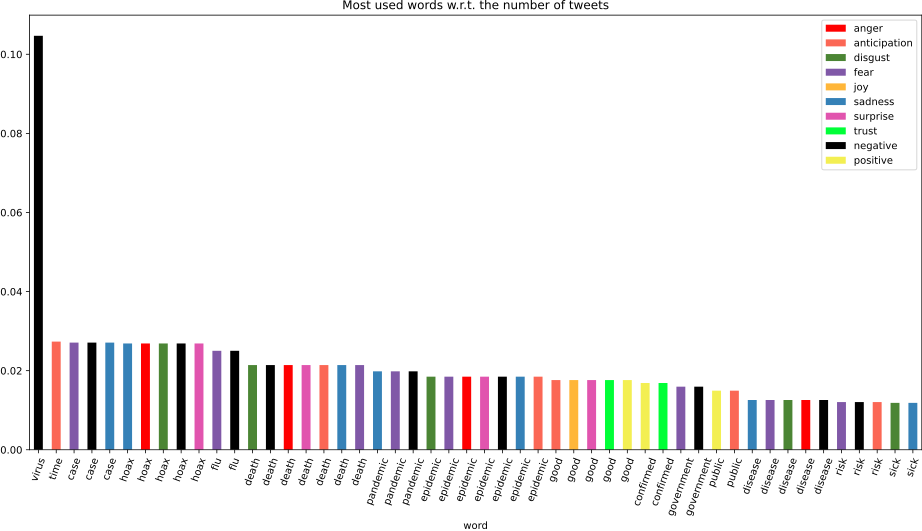
\includegraphics[scale=.32]{en_most_used_words_2020_02_24.svg}
    	\caption{Proportion of most used words on 2020/02/24 that express emotion/sentiment in the English tweets}
    	\label{fig:en-most-used-words-2020-02-24}
\end{figure}

Instead, \Cref{fig:en-most-used-words-2020-02-24} shows the results obtained from EmoLex for the same week.

First of all, we can notice that some words recognized by EmoLex are not identified by LIWC (and vice versa): for example, the word “virus”, which is present in the 10\% of the tweets. This happens because the word is either associated with a different category from the selected ones or is not present at all in the dictionary.

Secondly, some words, such as “virus”, are only related to a sentiment and not to any other emotion. On the other hand, “epidemic” is associated with almost the totality of the emotions. This is particularly problematic, because the course of the emotions tends to be all the same.

\section{Emotion detection over time - by gender}
\label{sec:emotion-by-gender-results}

\Cref{fig:en-4-categories-per-gender-course-mean} introduces the results of the analysis of the emotions expressed by females and males in the English tweets during the whole period. In this case, the dotted gray line represents the proportion of users that, independently from the category they belong to, expressed a certain emotion on a given week. However, this line differs from the results obtained in \Cref{fig:en-4-liwc-categories-subplots}, because we are now considering only the users with a certain number of tweets (see \Cref{subsec:m3inference} for further details).

We can also see that women tend to write a lot more tweets that convey sadness. This seems to be also the case for anxiety and positive emotions. However, probably because the words that express a positive emotion are used in many other context (e.g. “well”, “please”, “thank”, \ldots), the difference is less marked. Instead, men seem to express slightly more anger over the considered period, but the two lines overlap on more than one occasion.

\begin{figure}[H]
	\centering
    	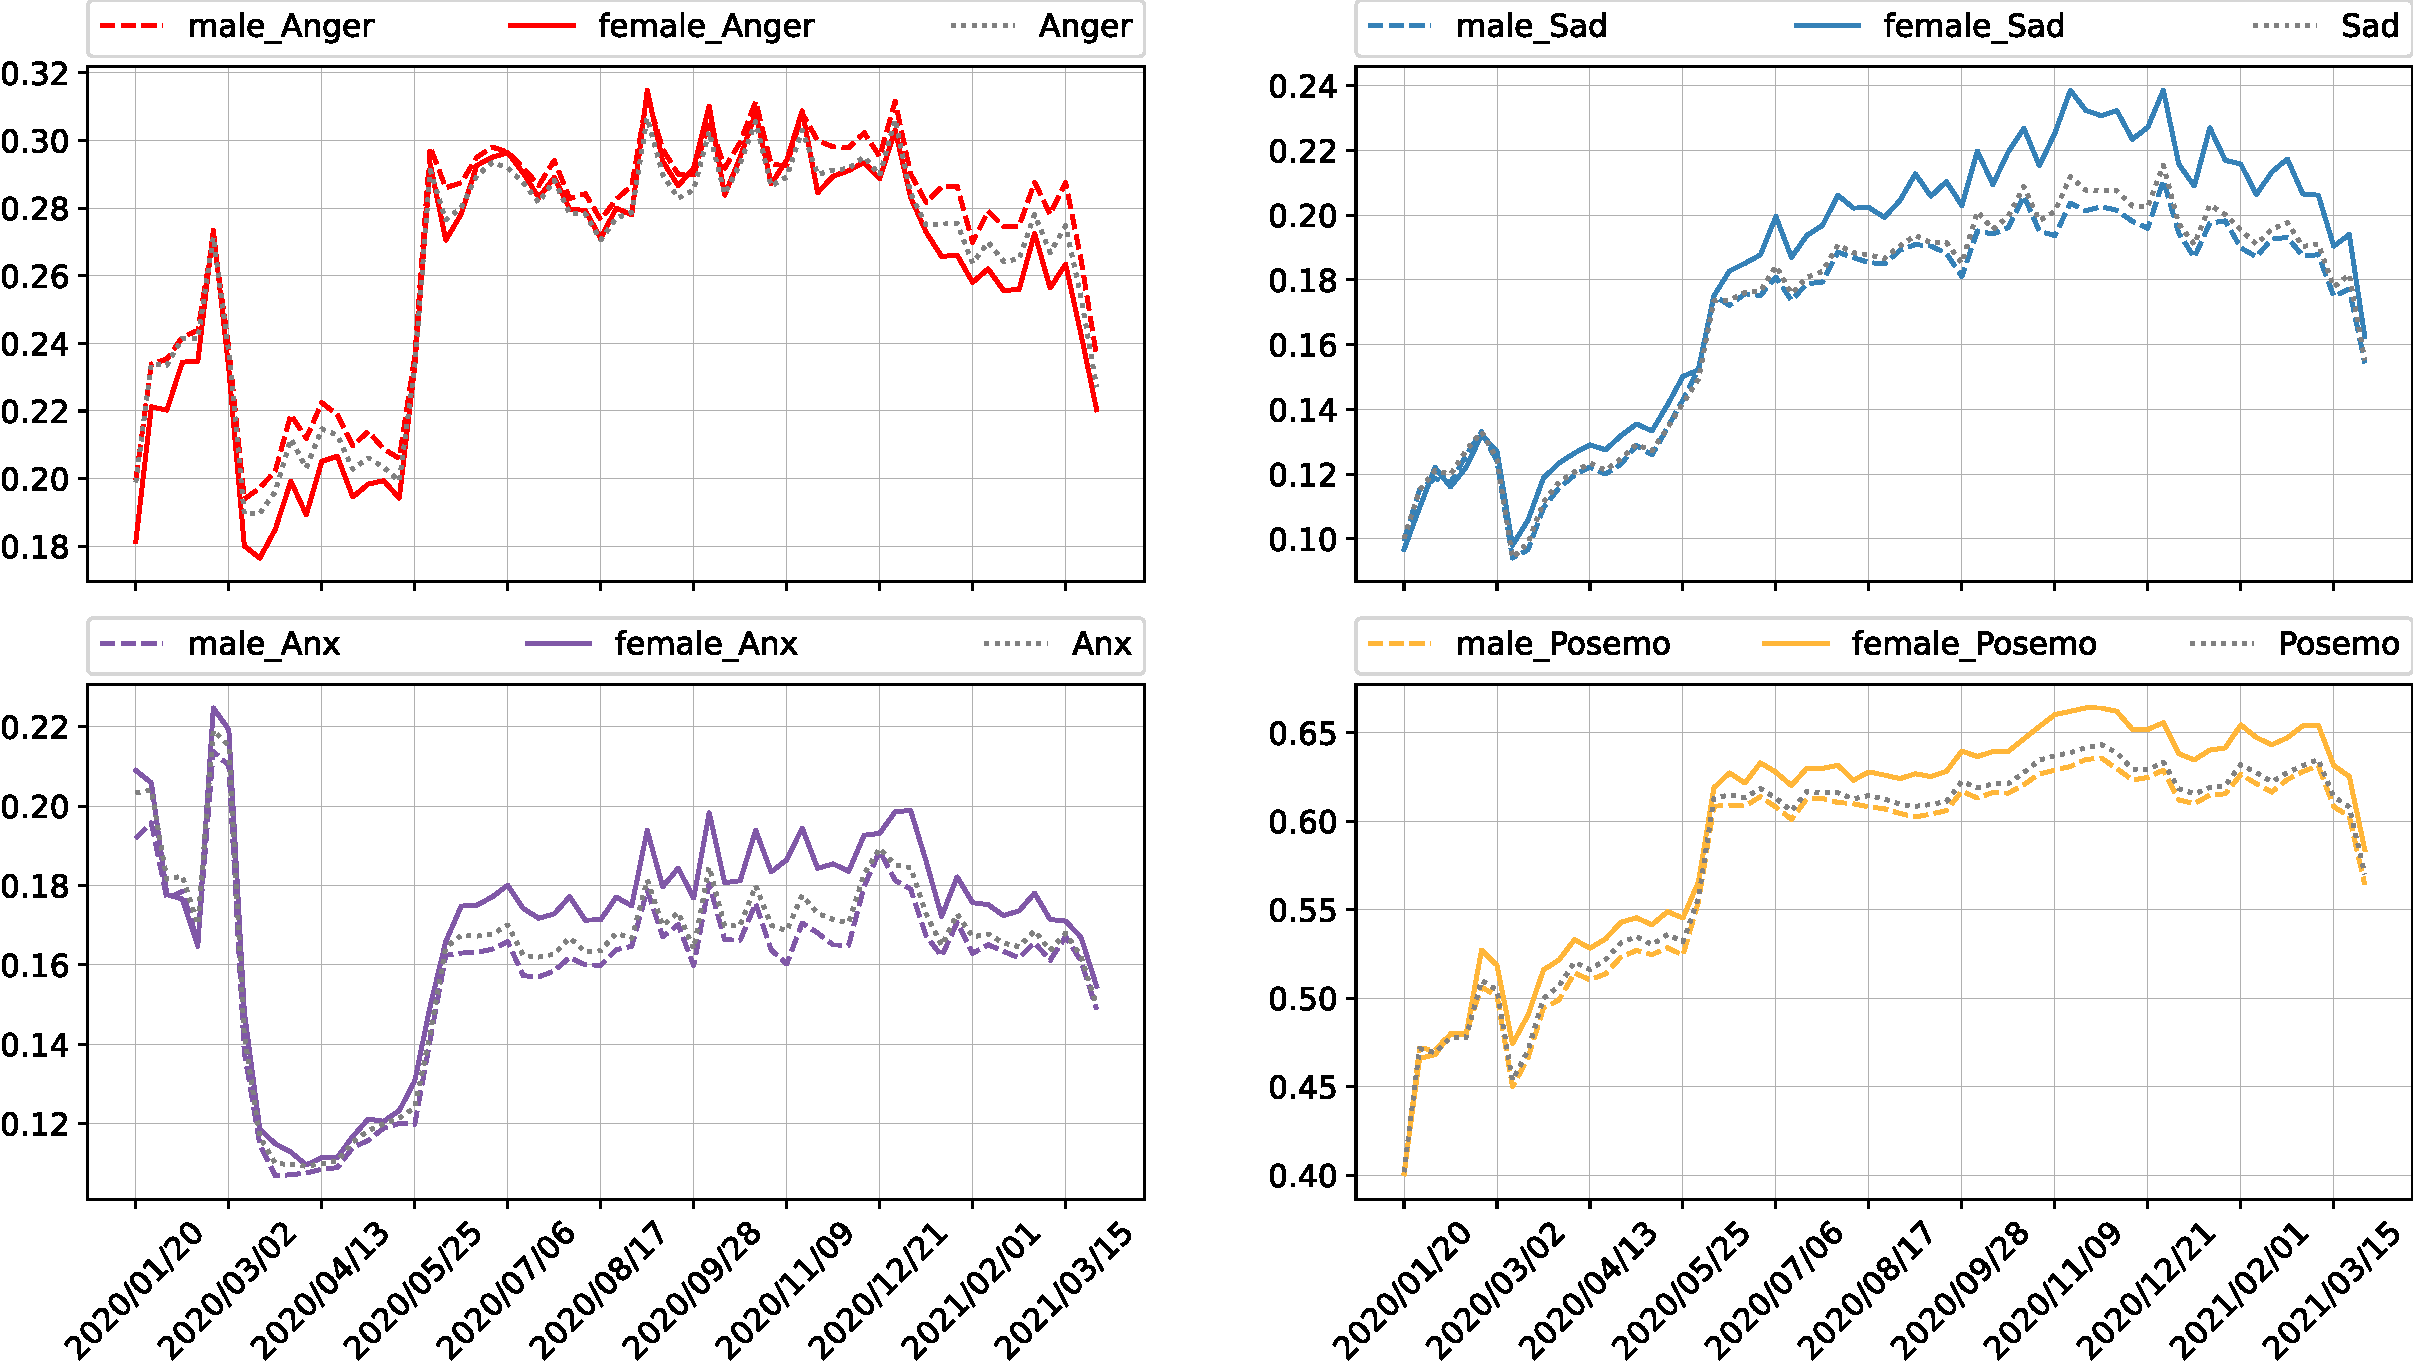
\includegraphics[scale=.35]{en_4_categories_per_gender_with_course_subplot.svg}
    	\caption{Proportion of weekly men/women expressing a particular emotion in the English tweets}
    	\label{fig:en-4-categories-per-gender-course-mean}
\end{figure}

\begin{figure}[H]
	\centering
    	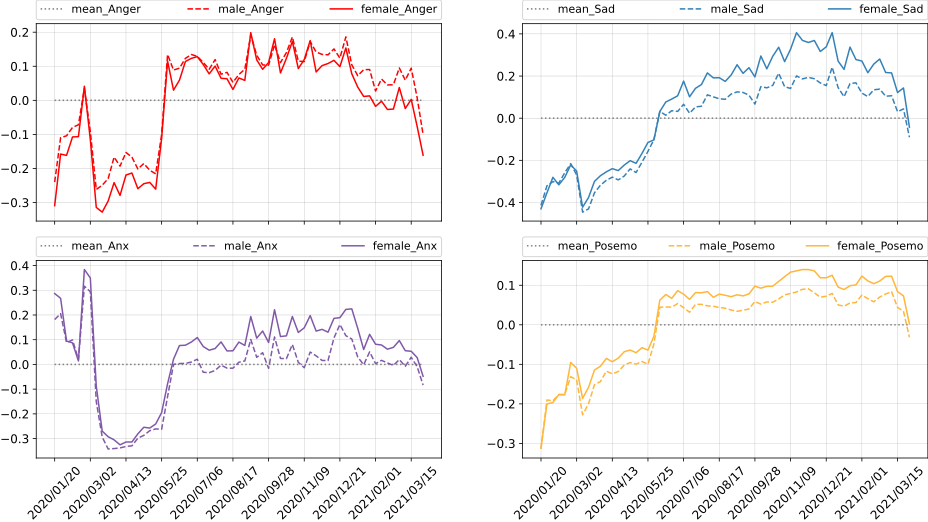
\includegraphics[scale=.35]{en_4_categories_per_gender_over_mean_subplot.svg}
    	\caption{Men/Women expressing the weekly proportion of a particular emotion w.r.t. the average value among all users}
    	\label{fig:en-4-categories-per-gender-over-mean}
\end{figure}

\Cref{fig:en-4-categories-per-gender-over-mean} is a variation of \Cref{fig:en-4-categories-per-gender-course-mean}, where the gray dotted line indicates the average value of a particular emotion expressed by all the users (i.e. independently from the category) over the whole period. Instead, the proportion reported by the other lines represents how much a certain gender expressed a particular emotion in a given week w.r.t. the mean value among the users. For example, both males and females expressed more or less 10\% less anger during the week starting on 2020/03/02.

\section{Emotion detection over time - by age}
\label{sec:emotion-by-age-results}

From the inference process, we also got information about age brackets.

\begin{figure}[H]
	\centering
    	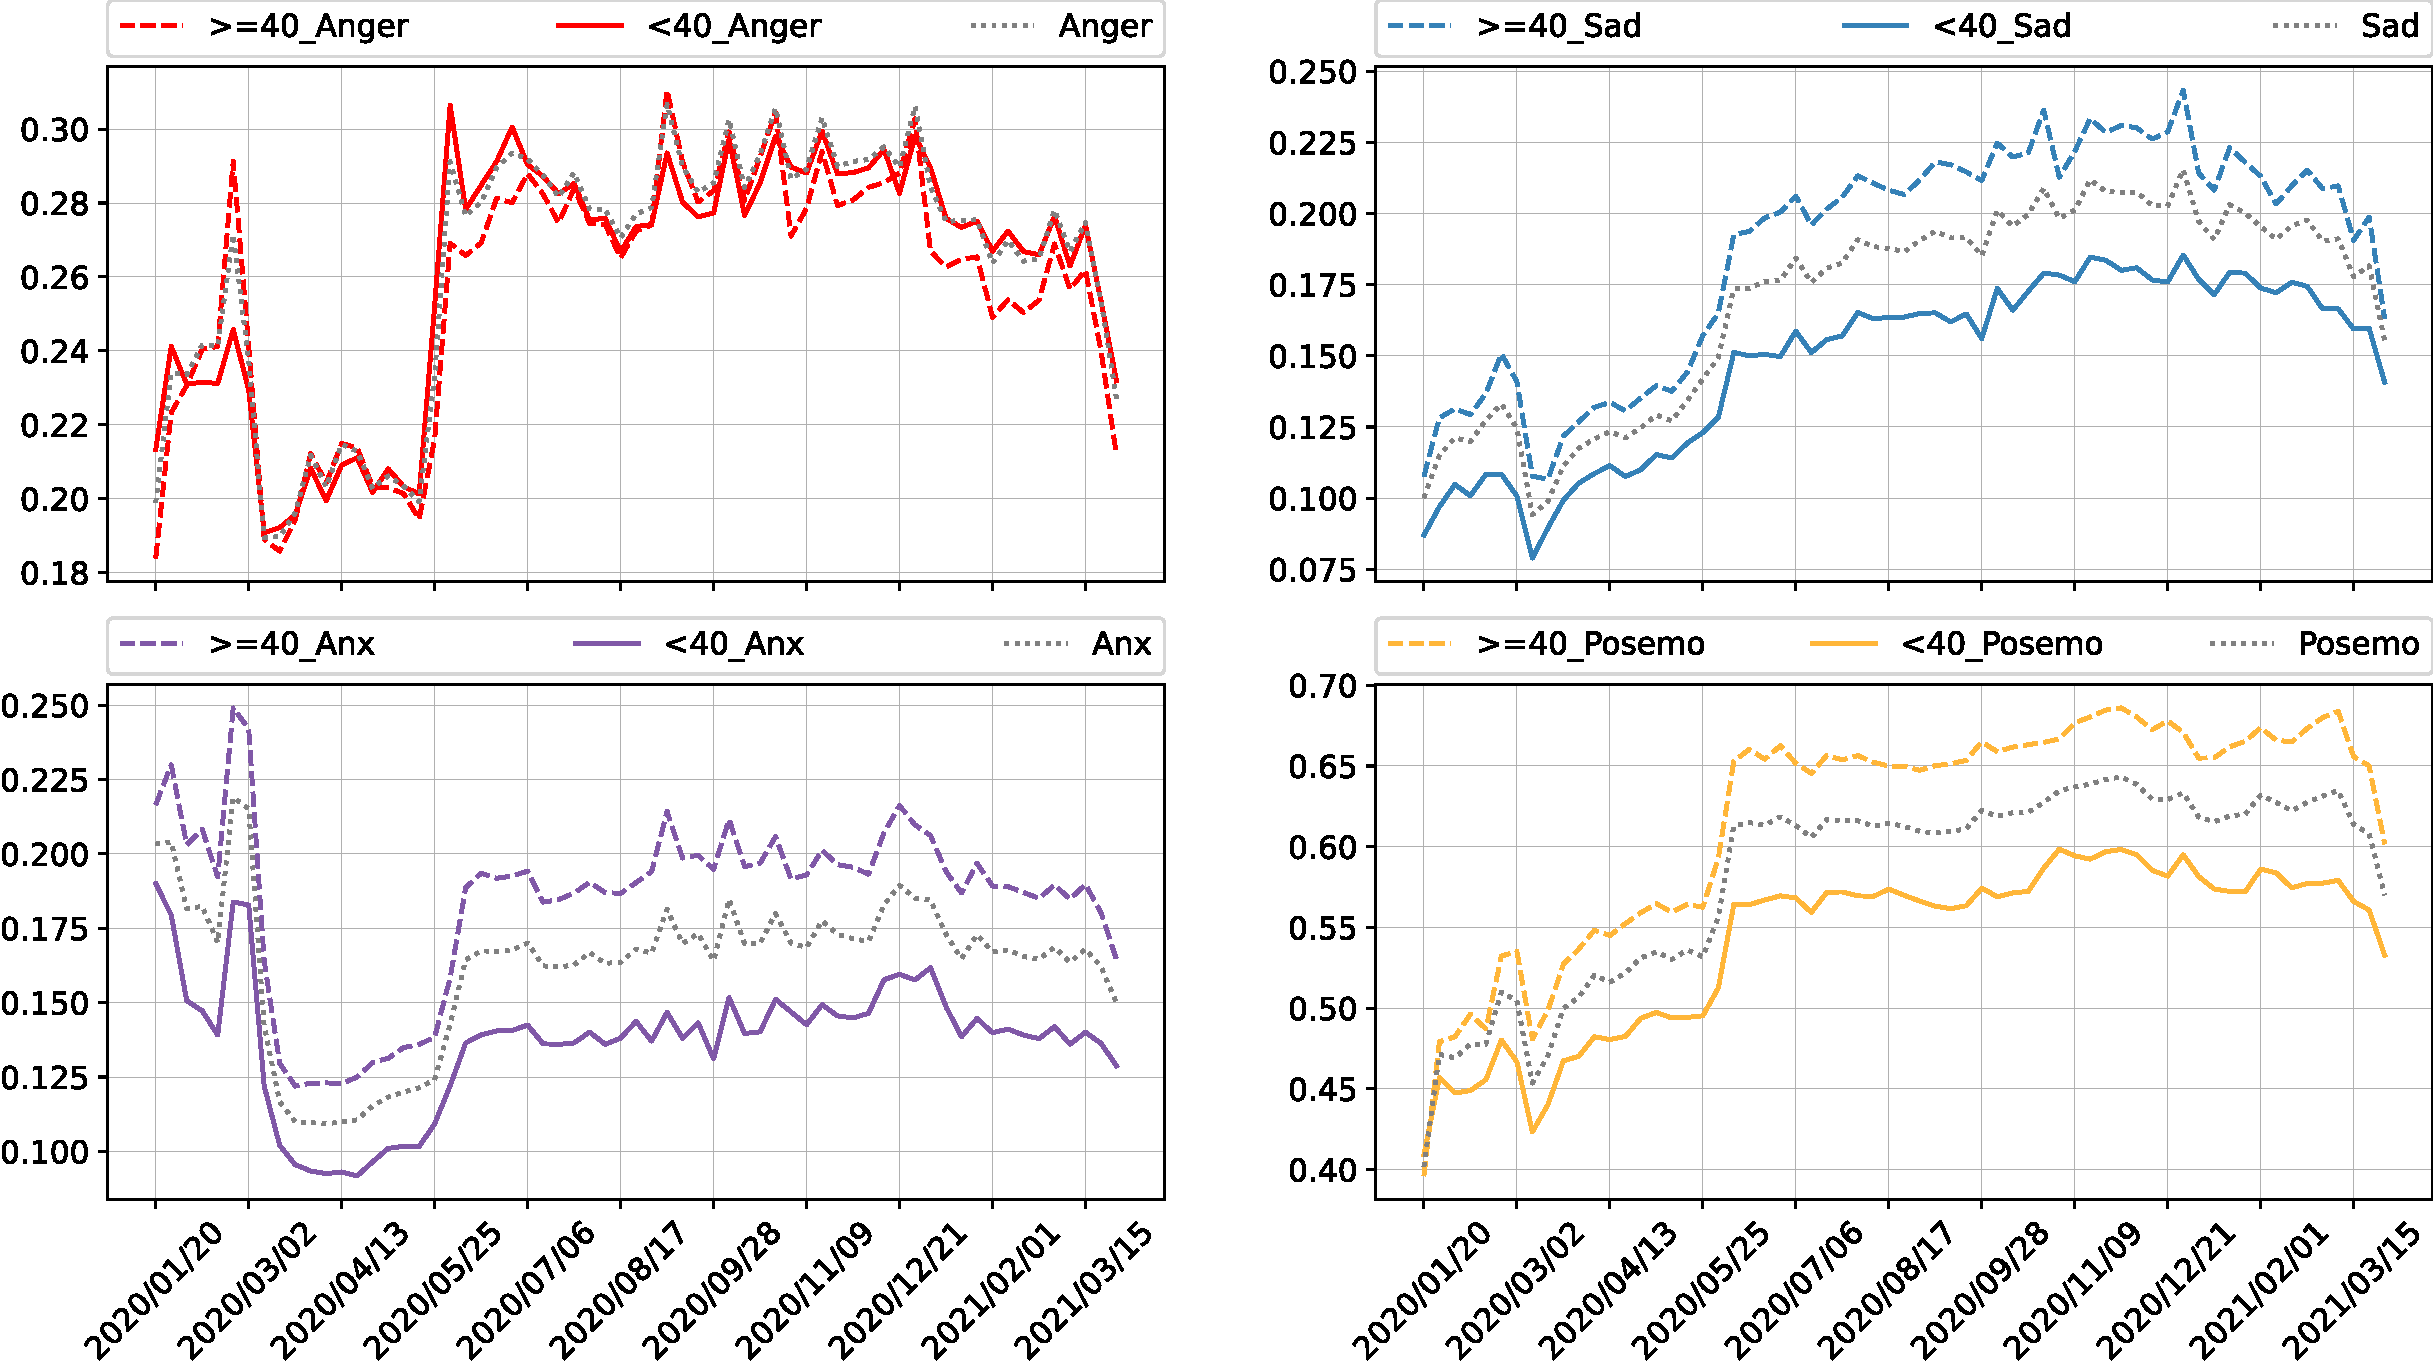
\includegraphics[scale=.35]{en_4_categories_per_age_with_course_subplot.svg}
    	\caption{Proportion of weekly users per age expressing a particular emotion in the English tweets}
    	\label{fig:en-4-categories-per-age-course-mean}
\end{figure}

\Cref{fig:en-4-categories-per-age-course-mean} shows the course of the emotions per age for the considered period. In particular, the dotted gray line represents the proportion of users that, independently from the age bracket they belong to, expressed a certain emotion on a given week. 

The results obtained are very intriguing because, in the case of sadness, anxiety, and positive emotions, there is always a noticeable gap between users below forty years old and those at least forty years old. However, that is not the case for anger. In fact, just like for men in \Cref{fig:en-4-categories-per-gender-course-mean}, users below forty years old seem to write tweets that convey slightly more anger.

To better understand this peculiar results, we decided to collect information about the number of users that did not express any emotion in their tweet. It turned out that \(14 \%\) of the users below forty years old did not express any emotion. This result is very interesting and could be caused by different reasons. For example, it may be possible that younger users like to write shorter tweets. In fact, with a very restricted set of words, it is likely to not express feelings at all. Besides, they could use different methods to convey their emotions, such through emoticons or slang: neither of them is in fact recognized by LIWC or EmoLex. Finally, it could also be the case that they are apathetic. 

\begin{figure}[H]
	\centering
    	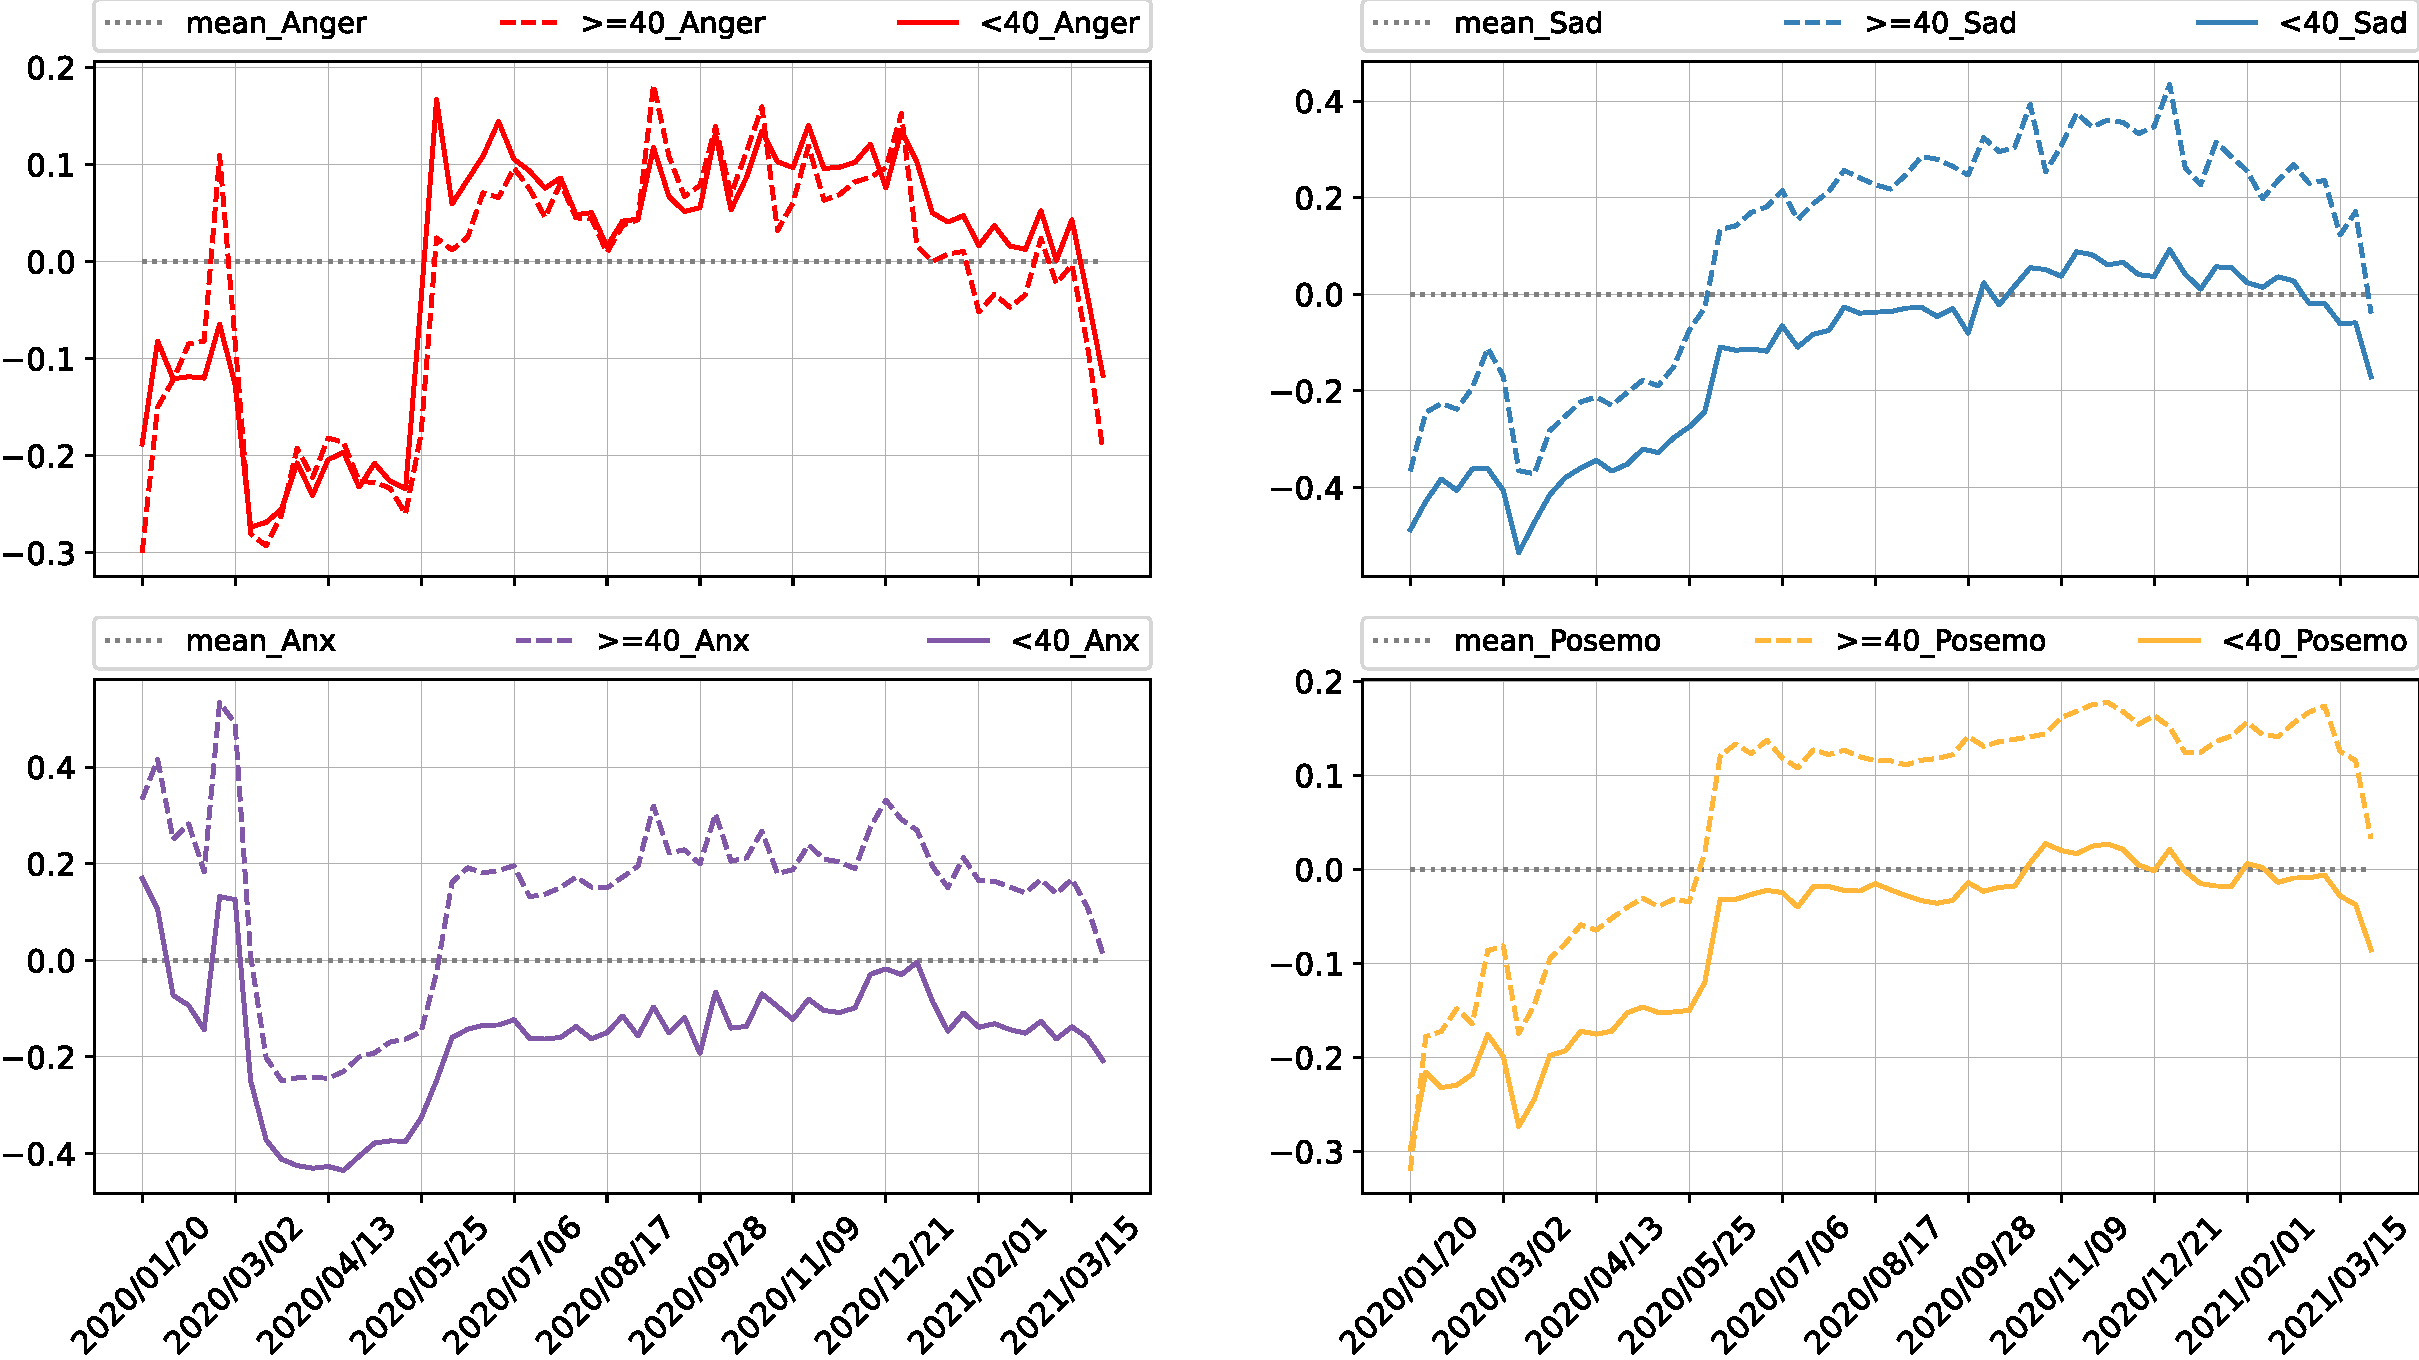
\includegraphics[scale=.35]{en_4_categories_per_age_over_mean_subplot.svg}
    	\caption{Users per age expressing the weekly proportion of a particular emotion w.r.t. the average value among all users}
    	\label{fig:en-4-categories-per-age-over-mean}
\end{figure}

Just like for \Cref{fig:en-4-categories-per-gender-over-mean}, \Cref{fig:en-4-categories-per-age-over-mean} is a variation of \Cref{fig:en-4-categories-per-age-course-mean}, where the gray dotted line indicates the average value of a particular emotion expressed by all the users (i.e. independently from the age bracket) over the whole period. Similarly, the proportion reported by the other lines represents how much a certain age bracket expressed a particular emotion in a given week w.r.t. the mean value among the users.


\section{Emotion detection over time - by location}
\label{sec:emotion-by-location-results}

Finally, we can now move to the analysis of the users' emotions from a specific location.

\Cref{fig:it-users-state} shows the proportion of users per region in Italy. From the results that we have obtained, we decided to consider only Lombardia, Lazio, Emilia Romagna, and Campania for further studies. In this way, we are able to better visualize the data and we have more possibilities to get stabler results.

From \Cref{fig:it-anger-4-states} we can actually understand which events had an impact on every region. For example, it is possible to notice a peak of anxiety during the week starting on 2020/02/17. The reason behind this is probably related to the first case of covid-19 found in Codogno.

\begin{figure}[H]
	\centering
    	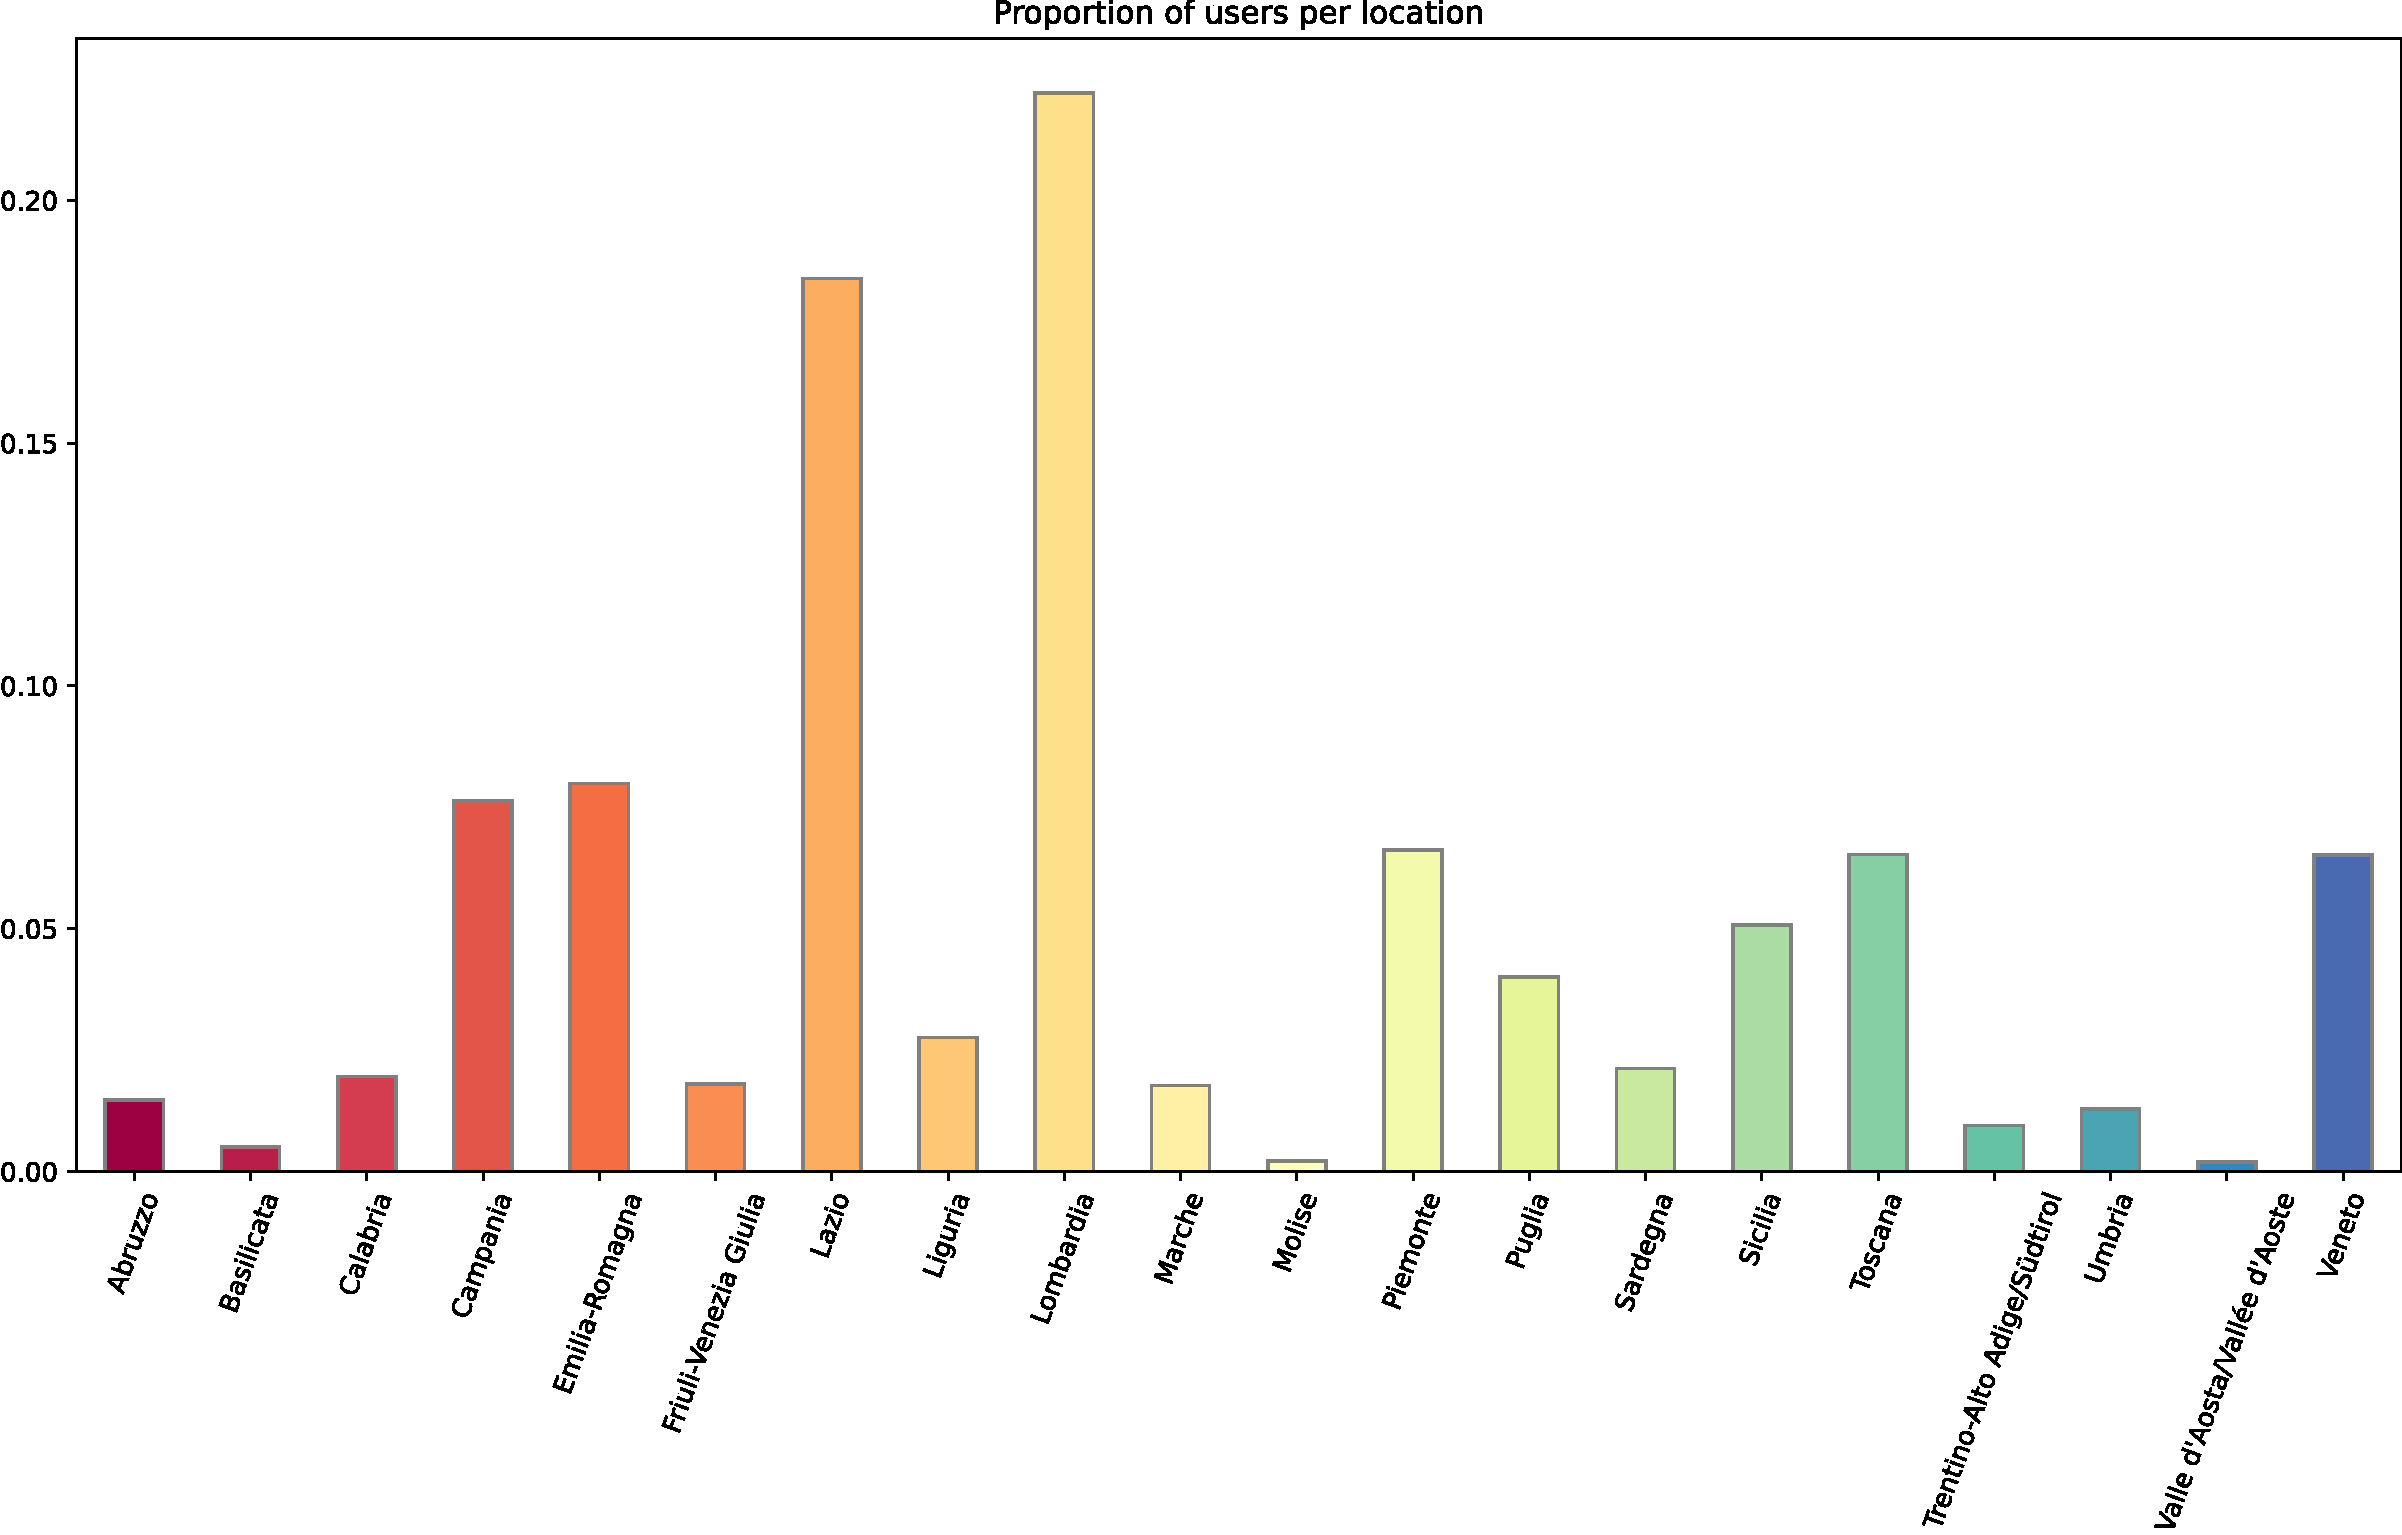
\includegraphics[scale=.35]{it_users_per_state.svg}
    	\caption{Proportion of users per region in Italy}
    	\label{fig:it-users-state}
\end{figure}

\begin{figure}[H]
	\centering
    	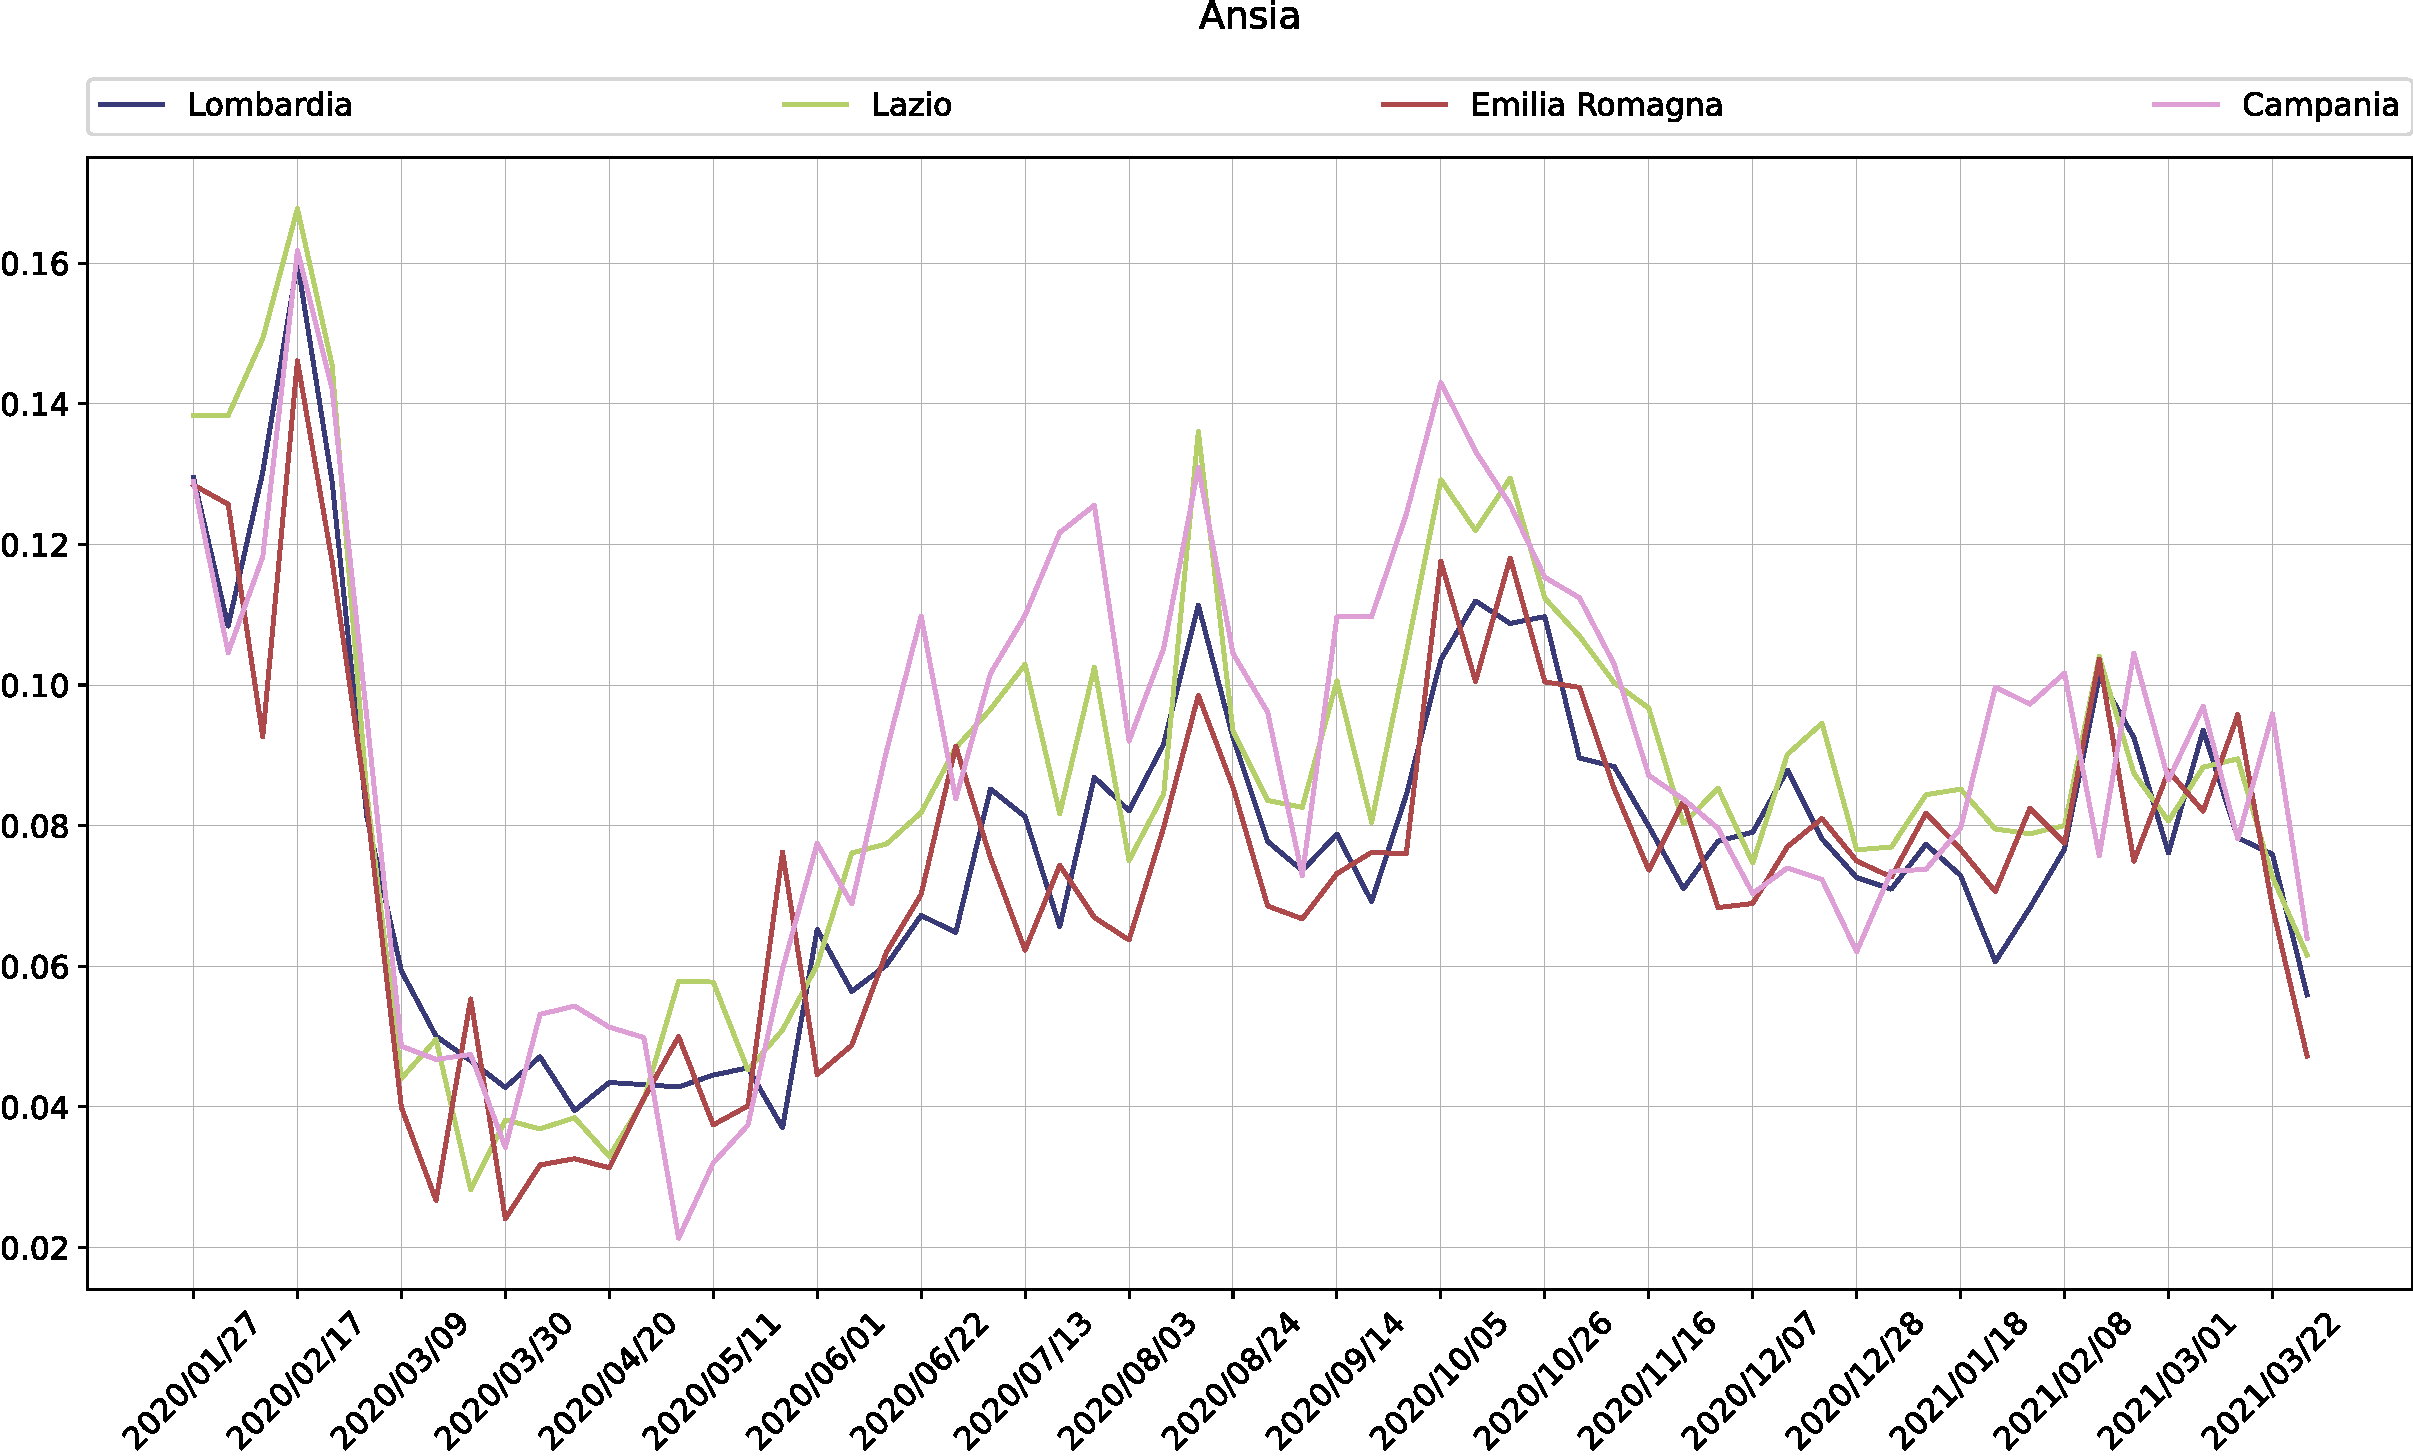
\includegraphics[scale=.35]{it_ansia_4_states.svg}
    	\caption{Proportion of weekly users that expressed anxiety in Lombardia, Lazio, Emilia Romagna and Campania}
    	\label{fig:it-anger-4-states}
\end{figure}

Of course, it is also possible to consider a single region, for example Lombardia, as showed in \Cref{fig:it-4-categories-lombardia}. Here we can notice even more how, by looking at the week starting on 2020/02/17, the news of the first coronavirus case in Codogno had an impact on people's emotions.

\begin{figure}[H]
	\centering
    	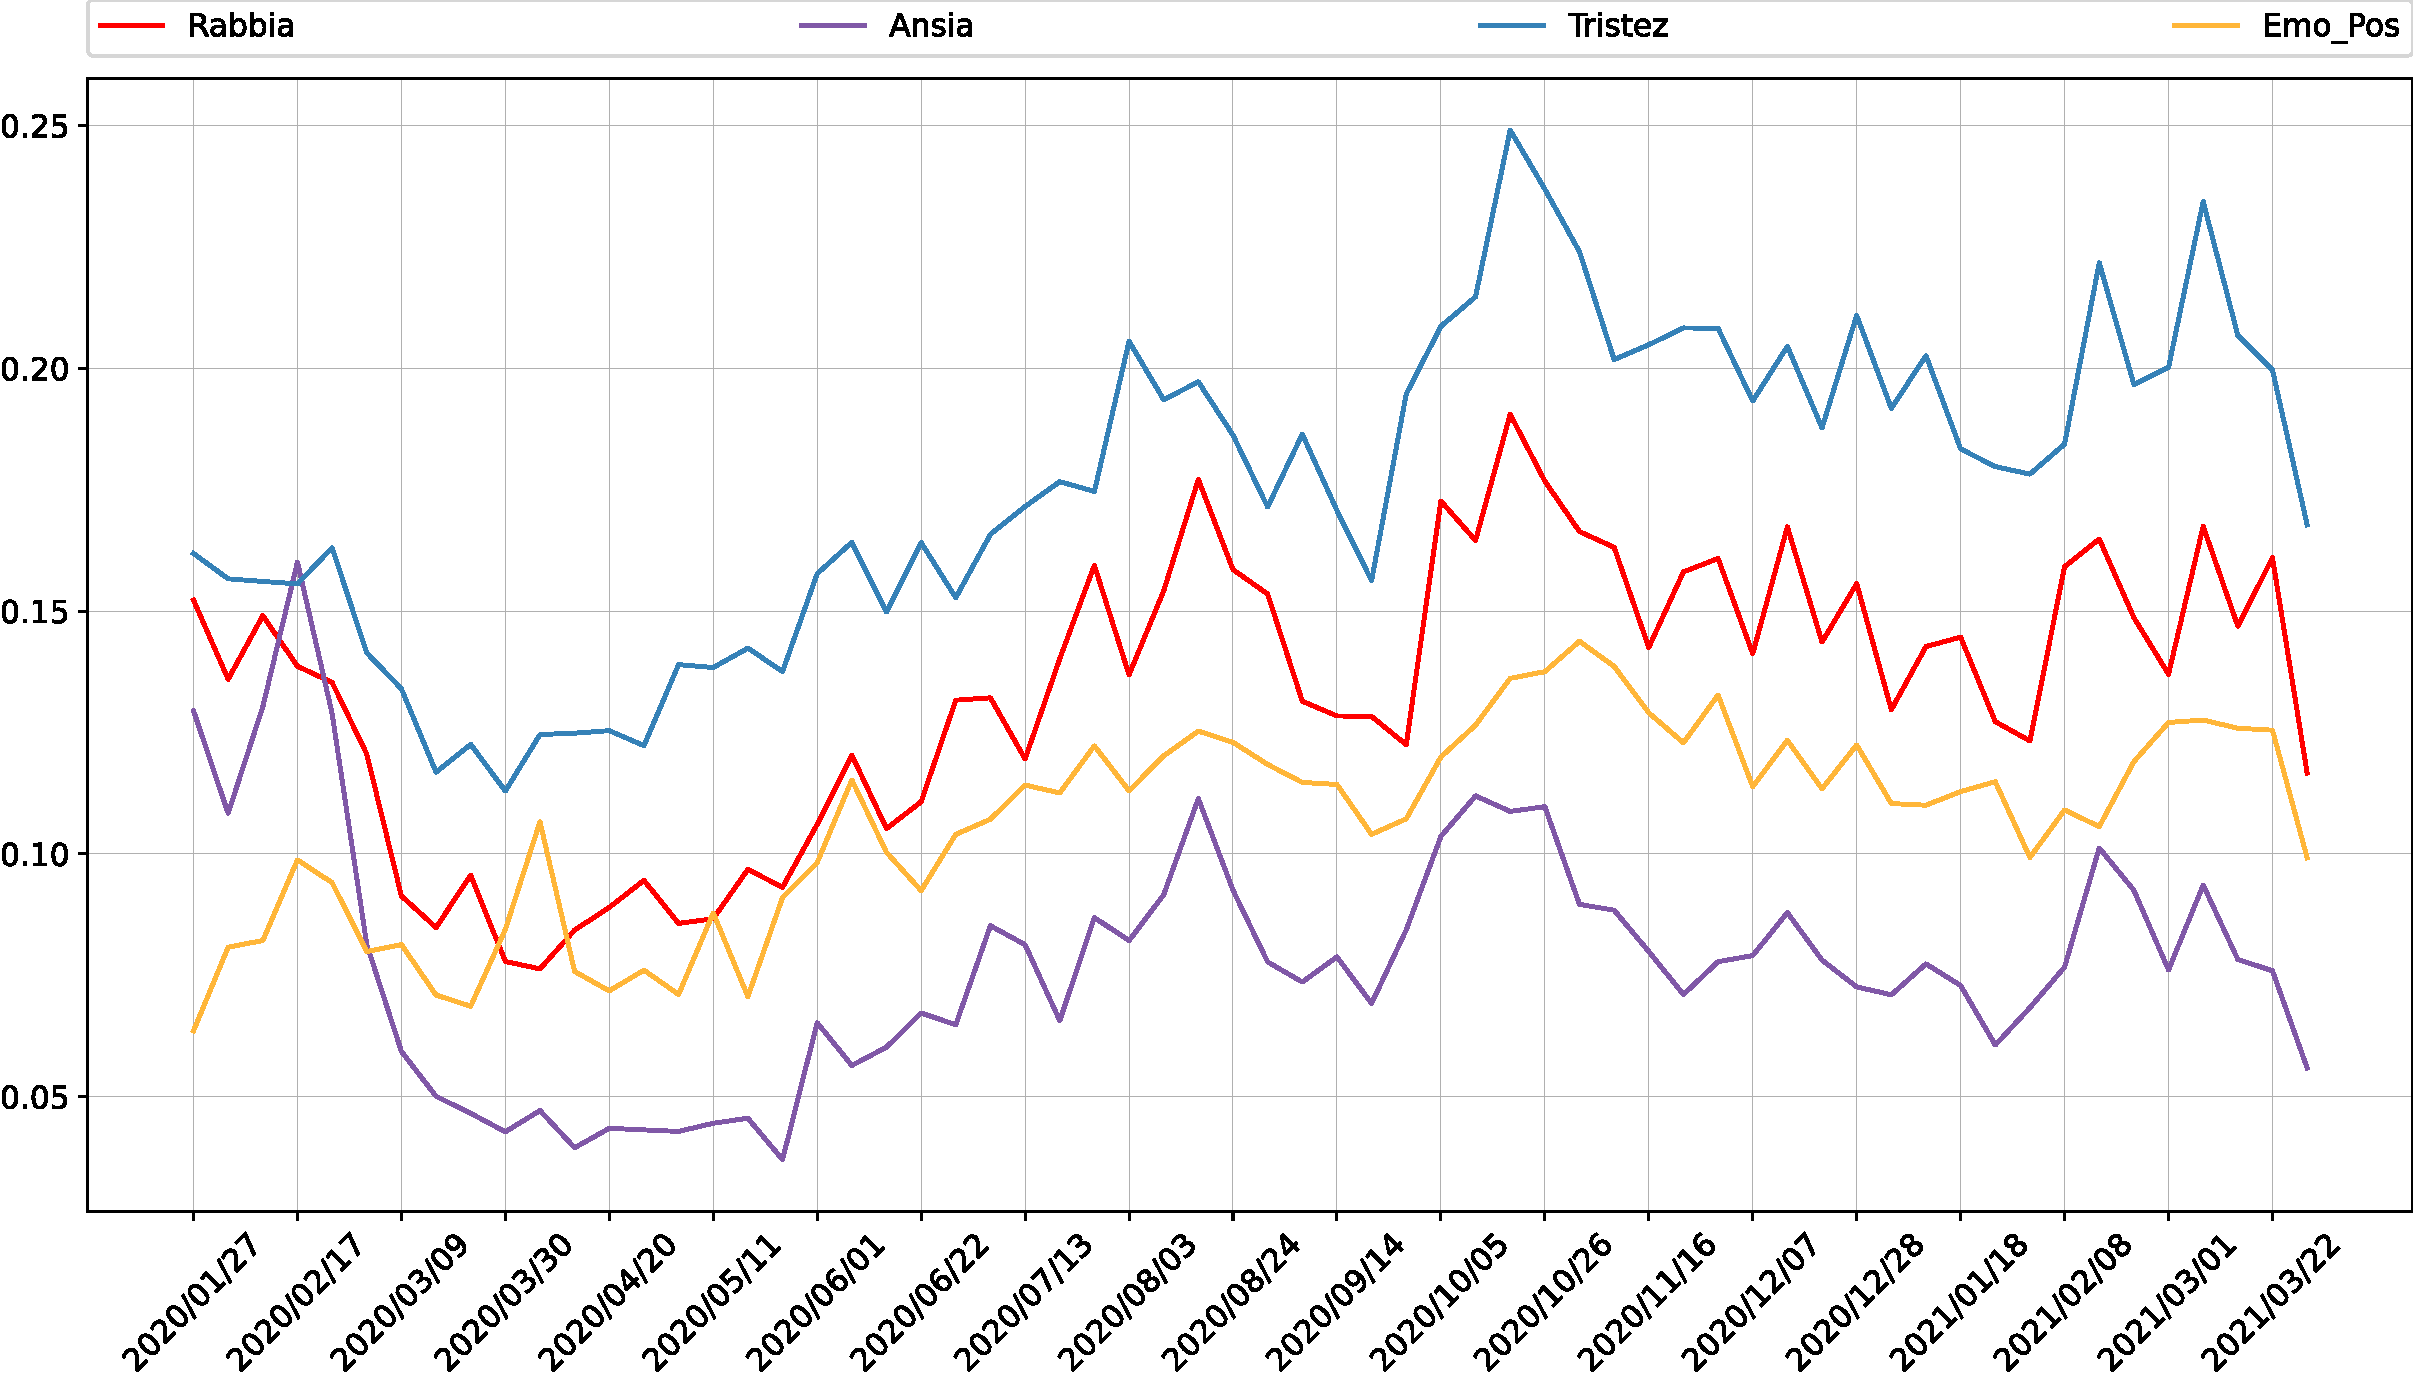
\includegraphics[scale=.35]{it_4_categories_lombardia.svg}
    	\caption{Proportion of weekly users per emotion in Lombardia}
    	\label{fig:it-4-categories-lombardia}
\end{figure}

\begin{figure}[H]
	\centering
    	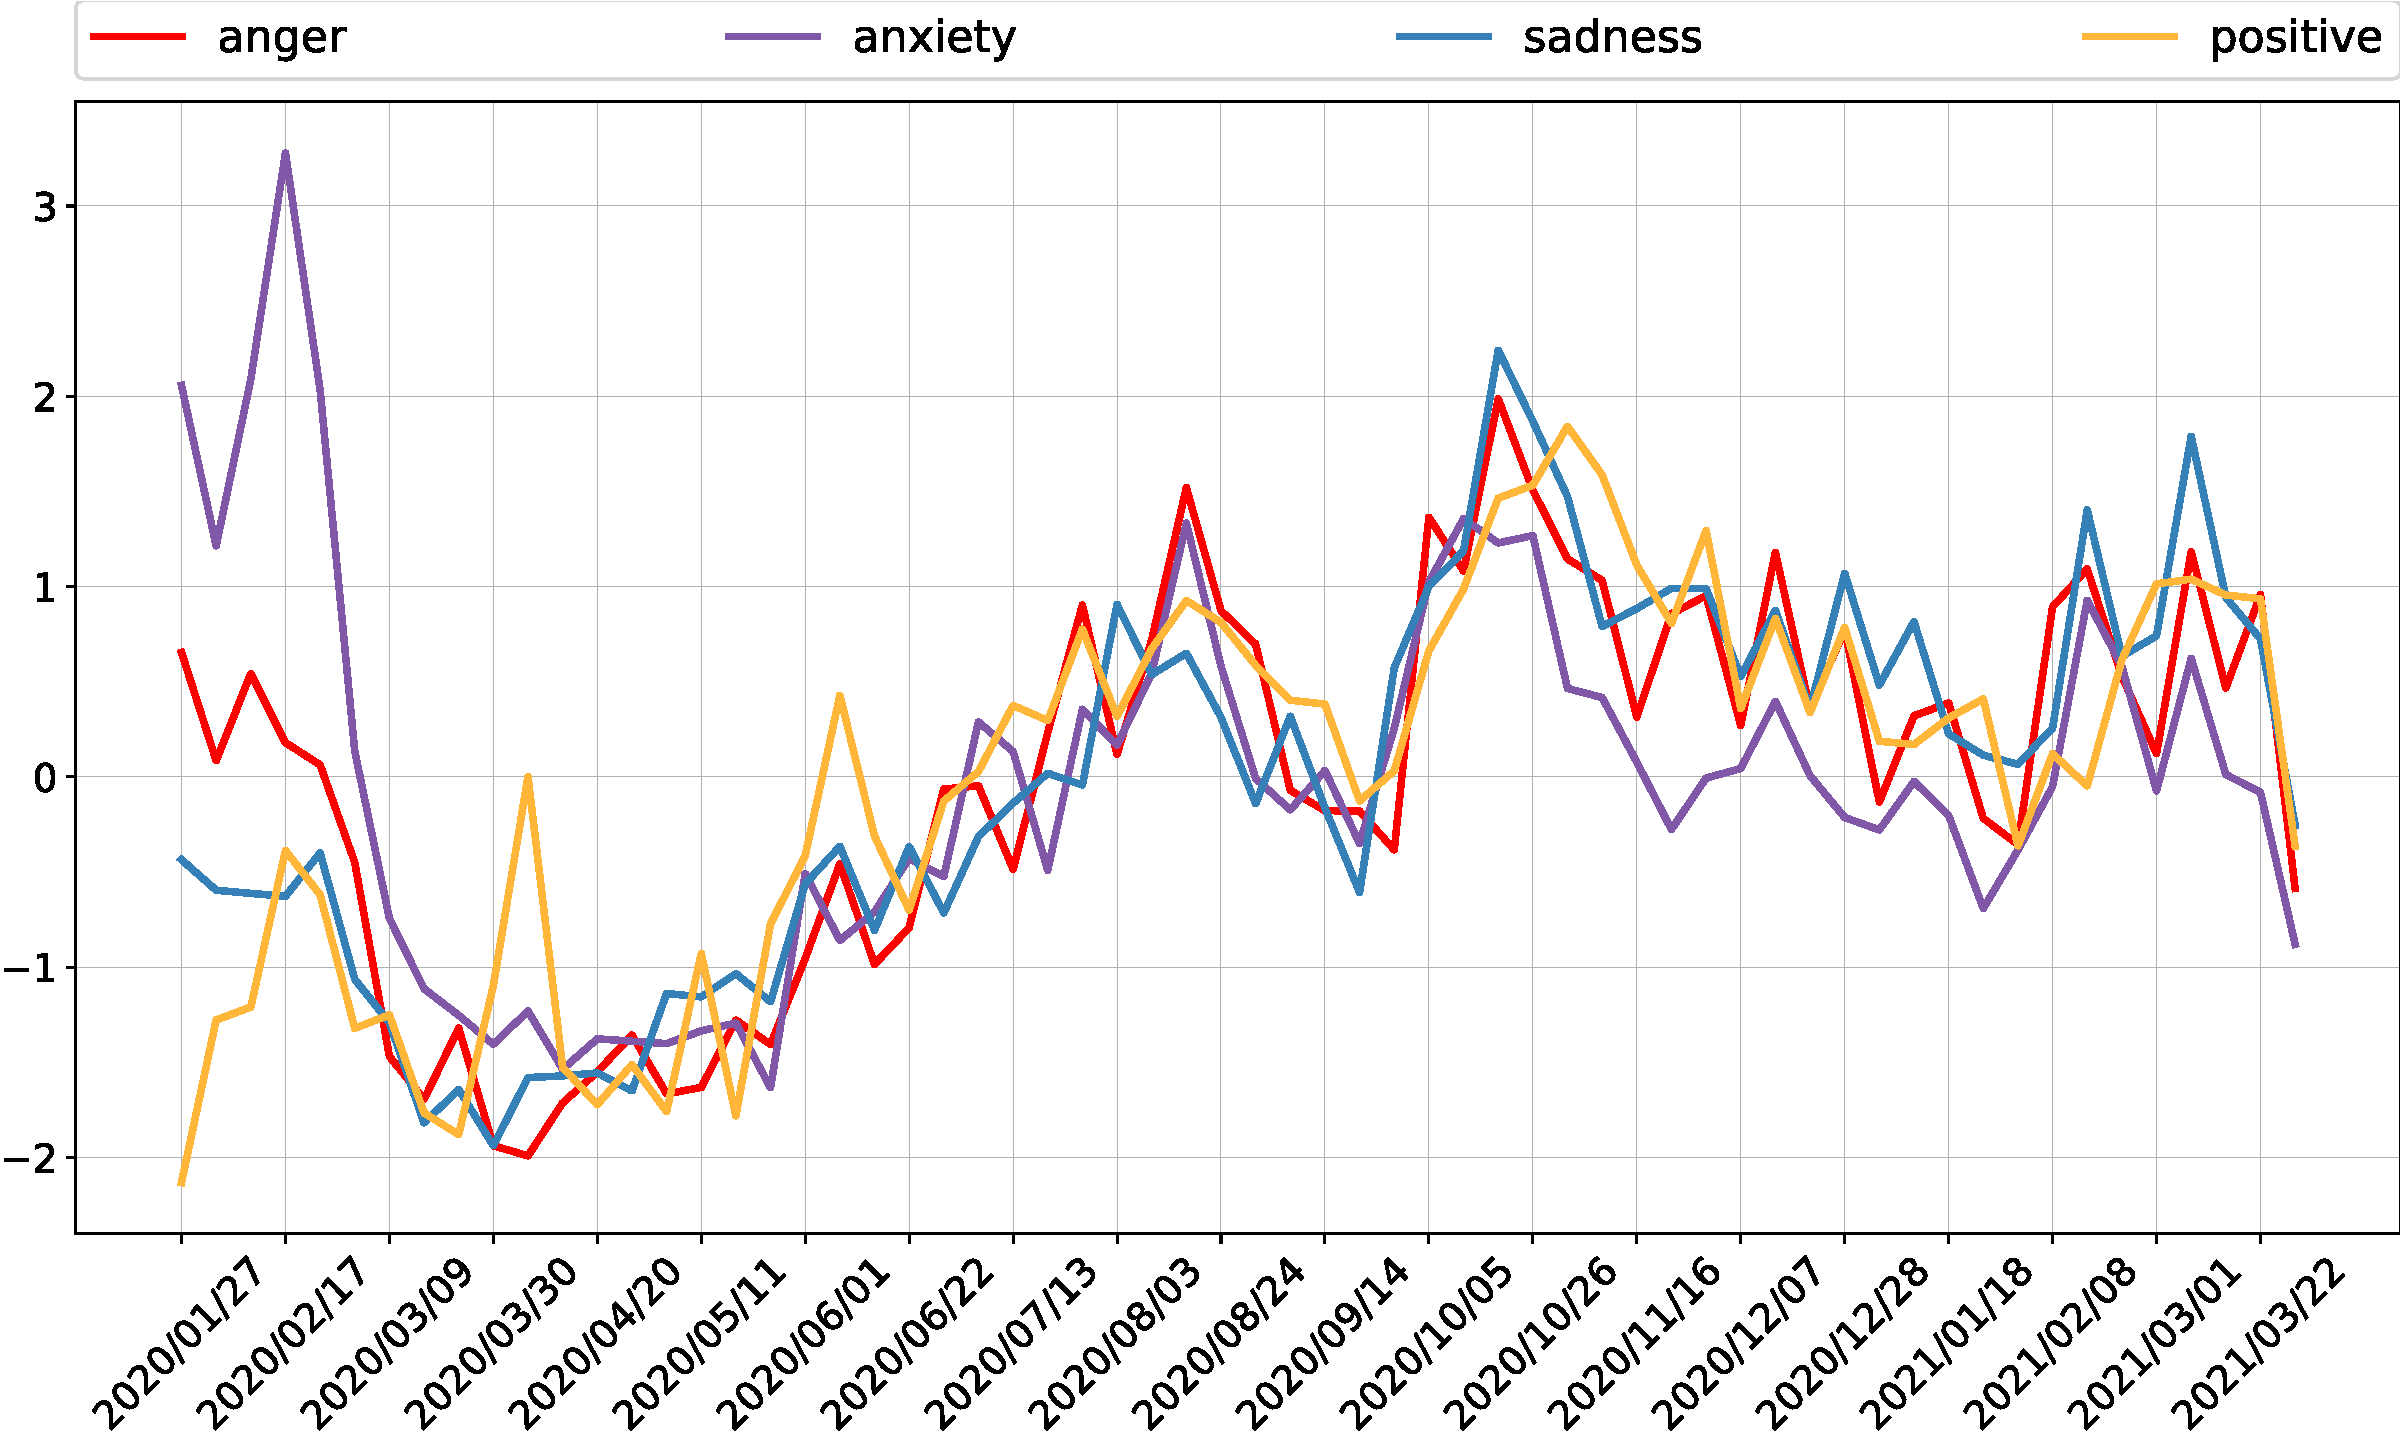
\includegraphics[scale=.35]{it_4_categories_lombardia_standardized.svg}
    	\caption{Z-score of weekly users per emotion in Lombardia}
    	\label{fig:it-4-categories-lombardia-std}
\end{figure}

The course of the emotion is even clearer if we look at the results obtained using the z-score. From \Cref{fig:it-4-categories-lombardia-std}, we can see how, after the first case, all the emotions decreased, probably because news and various decree helped to calm people down.

Instead, the peak of the positive emotions during the week of 2020/04/06 could be associated with Easter. In general, we can see how after the end of the first lockdown, the course of the emotions tends to raise.

Finally, the peak on 2020/10/19 could be associated with decree N. 623, which imposed different restrictions to slow the spread of the disease. In particular, the decree strengthened the rules emanated previously and obliged high schools to stop in presence activities.